\documentclass{article}
\usepackage[utf8]{inputenc}
\usepackage[margin=2cm]{geometry}
\usepackage{enumitem}
\usepackage{csquotes}

% maths packages
\usepackage{amsmath}
\usepackage{amssymb}
\usepackage{amsthm}
\usepackage{braket}

% remove space between ket and bra
\renewcommand\bra[1]{{\langle{#1}|}}
\makeatletter
\renewcommand\ket[1]{
  \@ifnextchar\bra{\k@t{#1}\!}{\k@t{#1}}
}
\renewcommand\ket[1]{
  \@ifnextchar\braket{\k@t{#1}\!}{\k@t{#1}}
}
\newcommand\k@t[1]{{|{#1}\rangle}}
\makeatother

% graphics packages
\usepackage{graphicx}
\usepackage{subcaption}
\usepackage[font={small,it}]{caption}
\usepackage{tikz}
\usetikzlibrary{positioning, circuits.logic.US}

% tikz ellipse arcs
\tikzset{
    partial ellipse/.style args={#1:#2:#3}{
        insert path={+ (#1:#3) arc (#1:#2:#3)}
    }
}

\title{Bernoulli Factories: Classical to Quantum}
\author{Suzie Brown \\ {\small supervised by Krzysztof \L atuszy\'nski}}
\date{\today}

% bibliography
\usepackage[round, sort&compress]{natbib}
\usepackage{har2nat} %%% Harvard reference style
\bibliographystyle{agsm}

% theorems
\newtheorem{thm}{Theorem}
\newtheorem{lemma}{Lemma}
\newtheorem{cor}{Corollary}
\theoremstyle{definition}
\newtheorem{defn}{Definition}
\newtheorem{examplex}{Example}
\newenvironment{example}
  {\pushQED{\qed}\renewcommand{\qedsymbol}{$\triangle$}\examplex}
  {\popQED\endexamplex}

% probability symbols
\newcommand{\PR}{\mathbb{P}}
\newcommand{\E}{\mathbb{E}}
\newcommand{\V}{\operatorname{Var}}
\newcommand{\iidsim}{\overset{iid}{\sim}}
\newcommand{\eqdist}{\overset{d}{=}}

% distributions
\newcommand{\Bern}{\operatorname{Bernoulli}}
\newcommand{\Geom}{\operatorname{Geom}}

% project-specific commands
\newcommand{\A}{\mathcal{A}}
\newcommand{\AND}{{\footnotesize AND }}
\newcommand{\NAND}{{\footnotesize NAND }}
\newcommand{\OR}{{\footnotesize OR }}
\newcommand{\NOR}{{\footnotesize NOR }}
\newcommand{\NOT}{{\footnotesize NOT }}

\begin{document}
\maketitle

\section{Introduction}
Loosely speaking, a Bernoulli factory is an algorithm taking $p$-coin flips (i.e.\ $\Bern(p)$ samples) as inputs and producing an $f(p)$-coin flip as output, where $p$ is unknown and $f$ is a known function. This idea is explained more thoroughly in Section \ref{sec:BFs}.
The existence and performance of such algorithms for various choices of $p$ has been a subject of interest since the 1950s when (pseudo-)random number generation was emerging, and a subject of focused study since the 1990s.

Bernoulli factories are necessary components of certain Monte Carlo strategies, particularly for calculating Metropolis-Hastings acceptance probabilities in pseudo-marginal methods and diffusion models. 
In both cases, some terms in the acceptance probability cannot be evaluated, but can be Bernoulli-sampled. Luckily the acceptance probability $\alpha$ does not need to be explicitly calculated; the Metropolis-Hastings accept/reject step only requires a $\Bern(\alpha)$ sample. Choosing whether to accept or reject a proposal therefore comes down to converting the available Bernoulli samples to the desired $\Bern(\alpha)$ sample, which is precisely a Bernoulli factory problem.

The fundamental problem of which functions are possible was neatly solved by \citet{keane1994}, who found necessary and sufficient conditions on $f$ for the existence of a Bernoulli factory, but their work does not address the question of running time (that is, the number of $p$-coin flips required as inputs).
Theorems of \citet{nacu2005} determined further conditions on $f$ for the running time to satisfy various properties.

The contribution of \citet{dale2015} is a theorem analogous to that of \citet{keane1994}, in the context of a `quantum Bernoulli factory': where the inputs are a quantum analogue of $p$-coins (`quoins'), and quantum processing is allowed.
They show that quantum algorithms can simulate a strictly larger class of functions than classical ones and, for classically simulable algorithms, may require many fewer input quoins than their classical counterparts do coins.

% general overview of the field of quantum monte carlo (quantum MH, qunatum MCMC etc?)

The remainder of the document is organised as follows.
Section \ref{sec:quantum_info} provides the background in quantum information theory required to understand the quantum Bernoulli factory. 
Section \ref{sec:BFs} introduces the Bernoulli factory problem and summarises previous work on classical solutions, starting with some illustrative examples before laying down the theoretical results.
Section \ref{sec:quantum_advantage} explains the context in the quantum information literature of a quantum Bernoulli factory and explains how it works, with comparison to the classical case.
Finally, Section \ref{sec:discussion} discusses the scope of its implications.

\section{Quantum information}\label{sec:quantum_info}
This section is based on the course by Noah Linden (University of Bristol) and discussion with Thomas Hebdige and David Jennings (Imperial College London). For a comprehensive introduction see for example \citet{nielsen2002} or \citet{wilde2013}.

The basis of quantum mechanics is simply linear algebra in a Hilbert space. The definitions in Sections \ref{sec:hilbert_defn} to \ref{sec:linear_ops} are exactly what you would find in a linear algebra course, except for the notation. 
The famously strange aspects of quantum behaviour arise chiefly from the `rules of quantum mechanics' (Section \ref{sec:rules_of_qm}) pertaining to measurements. The majority of phenomena besides are described perfectly naturally by standard linear algebra, and are only counter-intuitive when one departs from the safety of mathematical abstraction and attempts to interpret quantum behaviour within the framework of the natural world, as perceived on a human scale. 
It is not surprising that such attempts should lead to confusion, since quantum mechanics is based on complex numbers and so diverges from human reality even at its very fundamentals.

\subsection{Dirac notation}
Dirac notation is a convenient way of denoting vectors such that it is easy to visually identify inner and outer products, and thus quickly recognise scalars, vectors and matrices:

\begin{itemize}
\item $\ket{v}$ denotes a column vector
\item $\bra{v}$ denotes a row vector
\item $\braket{u|v}$ denotes an inner product (resulting in a scalar)
\item $\ket{u}\bra{v}$ denotes an outer product (resulting in a matrix)
\end{itemize}
Additionally, $\overline{\alpha}$ denotes the complex conjugate of a scalar $\alpha$, and $U^\dag$ denotes the adjoint (conjugate transpose) of an operator $U$.

\subsection{Hilbert space}\label{sec:hilbert_defn}
A \emph{Hilbert space} is a vector space with an inner product $\braket{\cdot|\cdot}$ satisfying the following:
\begin{itemize}
\item $\bra{u} \left(\alpha\ket{v} + \beta\ket{w}\right) = \alpha\braket{u|v} + \beta\braket{u|w}$
\item $\braket{u|v} = \overline{\braket{v|u}}$
\item $\braket{v|v} \geq 0$ with equality if and only if $\ket{v}$ is the zero vector.
\end{itemize}

\subsection{Orthonormal bases}\label{sec:onb}
An \emph{orthonormal basis} of a Hilbert space $\mathcal{H}$ is a set of vectors $\{v_1,\dots,v_n\}$ in $\mathcal{H}$ such that:
\begin{itemize}
\item $\operatorname{span} \{v_1,\dots,v_n\} = \mathcal{H}$
\item $\braket{v_i|v_j} = \delta_{ij}$
\end{itemize}
We henceforth restrict to the Hilbert space $\mathbb{C}^2$, which is the state space of a single quantum bit (qubit), and is sufficient to describe the basics of quantum information. The \emph{computational basis} $\{\ket{0}, \ket{1}\} = \{(1,0)^T,(0,1)^T\}$ is taken as the canonical basis for $\mathbb{C}^2$ and is used wherever not specified otherwise. Since it is an orthonormal basis, every vector $\ket{v}$ in $\mathbb{C}^2$ has a unique representation
\begin{equation*}
\ket{v} = \alpha \ket{0} + \beta \ket{1} \equiv (\alpha,\beta)^T
\end{equation*}
for some $\alpha, \beta \in \mathbb{C}$. We will restrict ourselves to \emph{normalised} vectors, requiring that $|\alpha|^2 + |\beta|^2 = 1$.
We will also consider two vectors equivalent if they differ only by an overall phase, i.e.\ $\ket{u} \equiv \ket{v}$ if $\ket{u} = e^{i\theta}\ket{v}$ for some $\theta$, since it is impossible to distinguish between two such quantum states by any measurement.

To ensure coherency with the properties of the inner product, we have that
\begin{equation*}
\bra{v} = \overline{\alpha} \bra{0} + \overline{\beta} \bra{1}.
\end{equation*}
The inner product of $\ket{v} = \alpha \ket{0} + \beta \ket{1}$ with $\ket{u} = \gamma \ket{0} + \delta \ket{1}$ is therefore computed as
\begin{align*}
\braket{v|u} &= (\overline{\alpha}\bra{0} + \overline{\beta}\bra{1}) (\gamma\ket{0} + \delta\ket{1})\\
&= \overline{\alpha}\gamma\braket{0|0} + \overline{\alpha}\delta\braket{0|1} + \overline{\beta}\gamma\braket{1|0} + \overline{\beta}\delta\braket{1|1} \\
&= \overline{\alpha}\gamma + \overline{\beta}\delta.
\end{align*}
One alternative choice of orthonormal basis which is worth mentioning is given by $\{\ket{+},\ket{-}\}$, consisting of the states
\begin{align*}
&\ket{+} := \frac{1}{\sqrt{2}}(\ket{0} + \ket{1}) \\
&\ket{-} := \frac{1}{\sqrt{2}}(\ket{0} - \ket{1}).
\end{align*}

\subsection{Linear operators}\label{sec:linear_ops}
A linear operator is an operator with the property
\begin{equation*}
A \left(\alpha\ket{u} + \beta\ket{v}\right) = \alpha A\ket{u} + \beta A\ket{v}.
\end{equation*}
It is therefore fully defined by its action on an orthonormal basis. For instance, the quantum \NOT operator (usually denoted $X$) is defined by
\begin{align*}
& X\ket{0} = \ket{1} \\
& X\ket{1} = \ket{0}
\end{align*}
Equivalently, $X$ can be expressed as a matrix with respect to the computational basis:
\begin{equation*}
X = \begin{pmatrix}
0 & 1 \\ 1 & 0
\end{pmatrix}
\end{equation*}
In Dirac notation, operators are written in terms of outer products of basis states:
\begin{equation*}
X = \ket{0}\bra{1} + \ket{1}\bra{0}
\end{equation*}
We see that this is equivalent to the matrix form:
\begin{equation*}
X = \begin{pmatrix}1\\0 \end{pmatrix} \begin{pmatrix} 0&1 \end{pmatrix}
+ \begin{pmatrix}0\\1 \end{pmatrix} \begin{pmatrix} 1&0 \end{pmatrix}
= \begin{pmatrix} 0 & 1 \\ 0 & 0 \end{pmatrix} +  \begin{pmatrix} 0 & 0 \\ 1 & 0 \end{pmatrix}
= \begin{pmatrix} 0 & 1 \\ 1 & 0 \end{pmatrix}.
\end{equation*}
The action of $X$ on a general state $\ket{v} = \alpha \ket{0} + \beta \ket{1}$ can be calculated from any of these definitions. In Dirac notation:
\begin{align*}
X\ket{v} &= (\ket{0}\bra{1} + \ket{1}\bra{0})(\alpha \ket{0} + \beta \ket{1})\\
&= \alpha \ket{0}\braket{1|0} + \alpha \ket{1}\braket{0|0} + \beta \ket{0}\braket{1|1} +
\beta \ket{1}\braket{0|1}\\
&= \alpha \ket{1} + \beta \ket{0}.
\end{align*}

\begin{defn}
Let $U$ be a linear operator.
\begin{itemize}
\item $U$ is said to be \emph{self-adjoint} (or \emph{hermitian}) if $U^\dag = U$.
\item $U$ is said to be \emph{unitary} if $UU^\dag = U^\dag U = I$.
\end{itemize}
\end{defn}

For example, the operator $X$ is both self-adjoint and unitary. Crucially, unitary operators preserve normalisation, so they map states to states. It is also obvious that unitary transformations are always reversible (i.e.\ the inverse operator exists).

\subsection{Rules of Quantum Mechanics}\label{sec:rules_of_qm}
\begin{enumerate}
\item \emph{States} of a quantum mechanical system correspond to normalised vectors in Hilbert space, up to an overall phase.
\item \emph{Evolutions} of the system correspond to unitary operators.
\item \emph{Measurements} on quantum states correspond to self-adjoint operators --- see below.
\end{enumerate}

\subsubsection{Spectral theorem and measurement}\label{sec:quantum_mmt}
The outcome of a measurement depends on the current state of the system and the type of measurement performed (i.e.\ which self-adjoint operator is applied).
The spectral theorem states that every self-adjoint operator $A$ can be represented by its spectral decomposition
\begin{equation}\label{eq:operator_diag}
A = \sum_{i} \lambda_i P_i
\end{equation}
where $\{\lambda_1,\dots, \lambda_k\}$ is the set of \emph{distinct} eigenvalues of $A$, and $P_i$ is the \emph{projection} operator onto the eigenspace corresponding to eigenvalue $\lambda_i$.

When we measure a state $\ket{x}$ using operator $A$, the measurement outcome we observe is one of the eigenvalues of $A$. In particular, we observe $\lambda_i$ with probability $\bra{x} P_i \ket{x} = |P_i\ket{x}|^2$.
Making a measurement causes the system to collapse onto the eigenspace corresponding to the observed eigenvalue; that is, the state after measurement is proportional to $P_i \ket{x}$.\\

\begin{example}\label{ex:quantum_mmt}
To give a concrete example, let us consider again the operator $X$. This operator has eigenvalues $\pm 1$ corresponding to eigenvectors (or \emph{eigenstates} in quantum mechanics) $\ket{+}$ and $\ket{-}$ respectively.
Therefore $X$ admits the diagonal representation
\begin{equation*}
X= \ket{+}\bra{+} \,-\, \ket{-}\bra{-}
\end{equation*}
which is of the form \eqref{eq:operator_diag}.
Now suppose we make a measurement on the state $\ket{v} = \ket{0}$, using $X$.
The outcome of the measurement will be an eigenvalue of $X$: either $+1$ or $-1$. We observe the outcome $+1$ with probability
\begin{equation*}
\bra{v} P_{+1} \ket{v} = \braket{0|+}\braket{+|0} = 1/2
\end{equation*}
in which case the state after measurement is
\begin{equation*}
P_{+1} \ket{v} = \ket{+} \braket{+|0} \,\propto\, \ket{+}.
\end{equation*}
Similarly, with probability 1/2 we observe the outcome $-1$ and the state after measurement is $\ket{-}$.
\end{example}

In this example, the two outcomes are equally likely because the state $\ket{0}$ is `equidistant' from the two eigenstates of $X$. In general, outcomes that leave the state after measurement closer to the original state are more likely. This notion is formalised in Section \ref{sec:bloch_sphere}.

A particularly important type of measurement is measurement in the computational basis. In this case the self-adjoint operator used is $0\cdot \ket{0}\bra{0} +1\cdot \ket{1}\bra{1} = \ket{1}\bra{1}$.
Measuring a state $\ket{v}=\alpha\ket{0} + \beta\ket{1}$ in the computational basis returns 0 with probability $|\alpha|^2$ or 1 with probability $|\beta|^2$. This is useful in quantum computing algorithms because it deterministically converts the basis states $\ket{0}$ and $\ket{1}$ to their classical equivalents 0 and 1, ready for classical output.

\begin{figure}
\centering
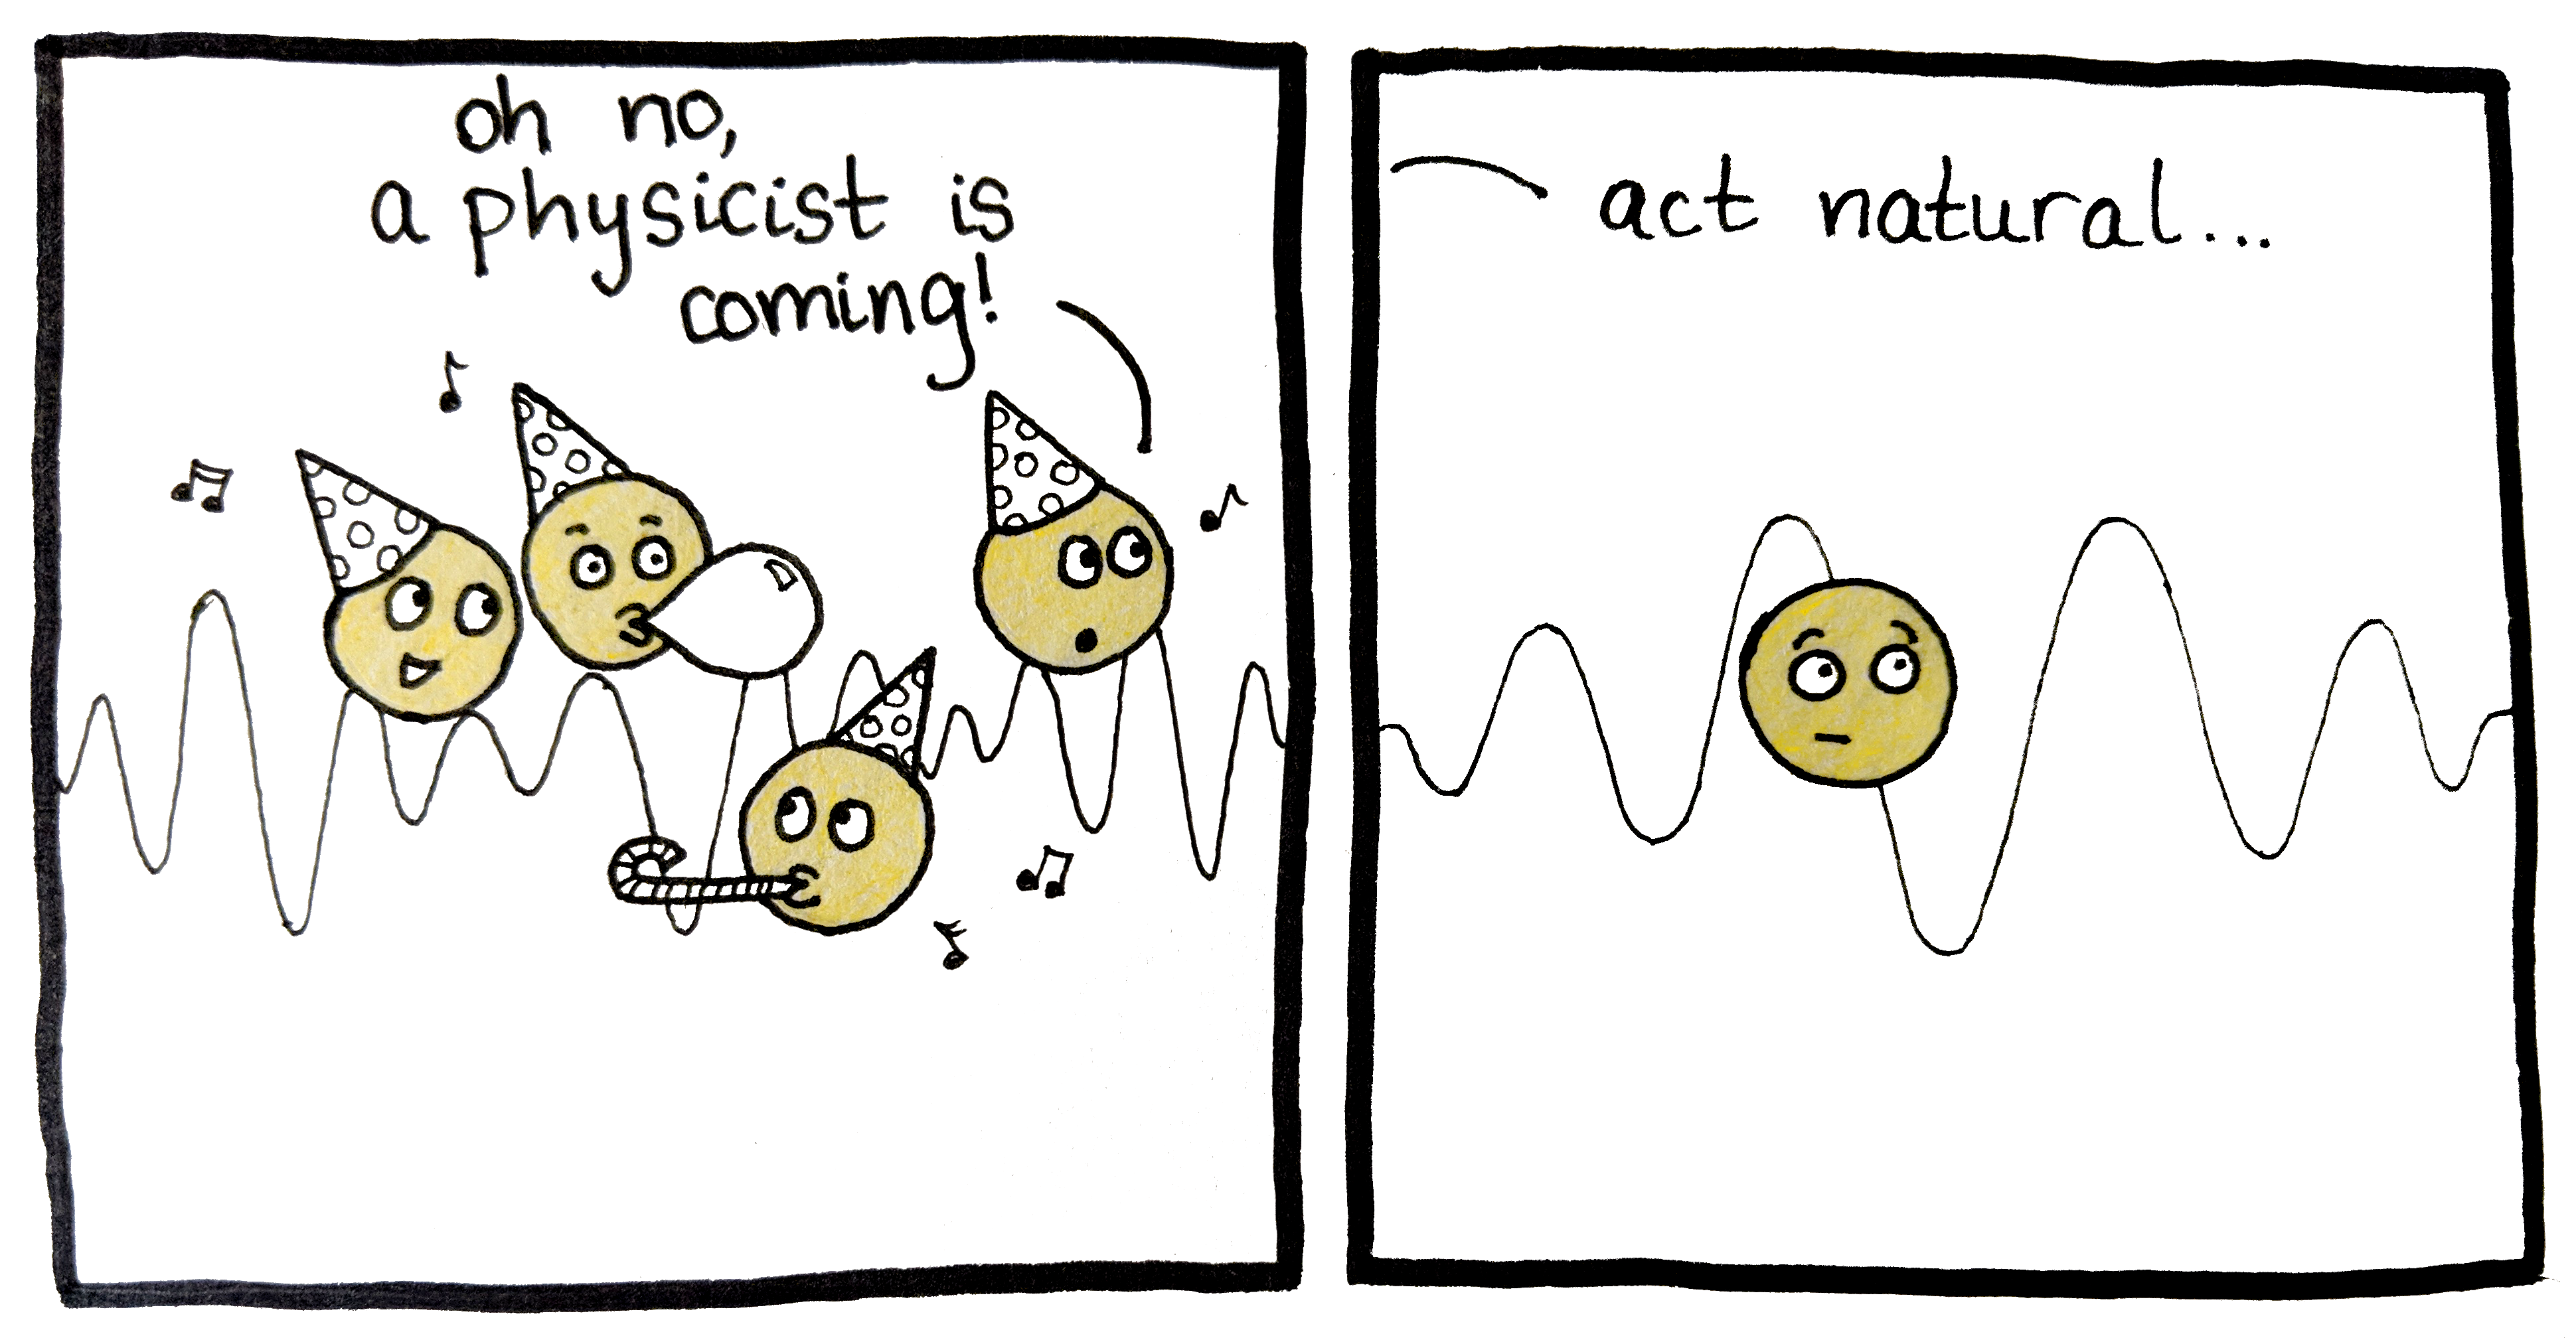
\includegraphics[width=0.8\textwidth]{qit_comic.png}
\caption{When a quantum system is in a superposition of states, making a measurement causes the system to collapse into the eigenstate corresponding to the observed eigenvalue.}
\label{fig:quantum_mmt_comic}
\end{figure}

\subsection{Quantum randomness}
It is worth remarking at this point on the difference between quantum and classical randomness.
As statisticians we are used to dealing with randomness, but we accept that randomness is simply part of a model, and is not purported to exist in nature. We artificially introduce random variables into our models to account for a lack of information, either about the state of the system or about the (presumably deterministic) processes that govern certain phenomena.

On the contrary, our uncertainty about the outcome of a measurement on a quantum system is of a different kind. This uncertainty is not a symptom of our lack of knowledge: even when we know exactly the state of the system, as in Example \ref{ex:quantum_mmt}, we are still unable to predict with certainty the outcome of a measurement on the system. The randomness here is intrinsic; the natural processes governing quantum measurement are truly stochastic.

\subsection{Pure and mixed states}
So far we have only encountered \emph{pure states}, like $\ket{0}$ or $\ket{+}$. But we can also consider probabilistic mixtures of pure states, known as \emph{mixed states}, like
\begin{equation*}
\ket{v} = \sum_{i} p_i \ket{v_i}
\end{equation*}
where $\{p_i\}$ is a probability distribution and the $\ket{v_i}$ are pure states.
You can think of this as a `source' which emits a state $\ket{v_i}$ with probability $p_i$.
A classical analogue is a bit that takes the value 1 with probability $p$ or 0 with probability $1-p$ (that is, a $p$-coin). In this case, we can say that the expected value of the bit is $p$.

There is no full ordering on the set of quantum states, so it is not possible to define the expected value of a mixed state. However, we can calculate the expected outcome of a measurement on a mixed state, using the state's \emph{density operator}.

\subsubsection{Density operators}
The density operator of a mixed state $\ket{v} = \sum_{i} p_i \ket{v_i}$ is given by
\begin{equation*}
\rho = \sum_{i} p_i \ket{v_i}\bra{v_i}.
\end{equation*}
Suppose we measure this mixed state using the self-adjoint operator $A= \sum_k \lambda_k P_k$, where $\{\lambda_k\}$ are the distinct eigenvalues of $A$ and $P_k$ the projections onto the corresponding eigenspaces. Recall (from Section \ref{sec:quantum_mmt}) that the outcome of the measurement will be an eigenvalue of $A$. Applying the law of total probability, the probability of observing a particular outcome $\lambda_j$ is
\begin{equation*}
\sum_i p_i \bra{v_i} P_j \ket{v_i} = tr(\rho P_j)
\end{equation*}
where $tr(\cdot)$ denotes the trace of an operator.
Note that $tr(\rho)=1$ because the states are normalised and $\{p_i\}$ is a probability distribution.
The state $\rho = I/2$ (where $I$ denotes the identity operator) is called the \emph{maximally mixed} state; it expresses complete ignorance, like a classical (1/2)-coin.

Different mixtures of states may have the same density operator, but in that case is is impossible to distinguish between them by any measurement. 
\begin{example}
For example, a source $\ket{u}$ that emits $\ket{0}$ or $\ket{1}$ each with probability 1/2 has the same density operator $\rho = I/2$ as a source $\ket{v}$ that emits $\ket{+}$ or $\ket{-}$ each with probability 1/2.
Suppose we measured both of these mixed states in the computational basis. The probability of observing the outcome 0 from $\ket{u}$ is
\begin{equation}
\bra{u}P_0\ket{u} = \frac{1}{2}\braket{0|0}\braket{0|0} + \frac{1}{2}\braket{1|0}\braket{0|1}
= \frac{1}{2}\cdot 1 + \frac{1}{2}\cdot 0= 1/2
\end{equation}
while the probability of observing 0 from $\ket{v}$ is
\begin{equation}
\bra{v}P_0\ket{v} = \frac{1}{2}\braket{+|0}\braket{0|+} + \frac{1}{2}\braket{-|0}\braket{0|-}
= \frac{1}{2}\cdot\frac{1}{2} + \frac{1}{2}\cdot\frac{1}{2}  = 1/2.
\end{equation}
Therefore measurement in the computational basis can provide no information to distinguish between $\ket{u}$ and $\ket{v}$. And indeed nor can any other measurement --- proved easily by exchanging the projection operator $\ket{0}\bra{0}$ for general $P$ in the above --- so the two sources are indistinguishable.
\end{example}

\subsection{The Bloch sphere}\label{sec:bloch_sphere}
Density operators have a neat geometrical representation as points in a unit sphere (Figure \ref{fig:qubit_state_space}). This is known as the \emph{Bloch sphere}, and can be thought of as the state space of a qubit.

An arbitrary pure state can be written in the form
\begin{equation*}
\ket{v} = e^{i\psi} \left[ \cos \left(\frac{\theta}{2}\right) \ket{0} + e^{i\phi} \sin \left(\frac{\theta}{2}\right) \ket{1} \right].
\end{equation*}
Since the overall phase $e^{i\psi}$ can be ignored, the state is parametrised by two angles $\theta$ and $\phi$. Taking these as spherical coordinates with unit radius, we can think of each pure state as a point on the unit sphere (or equivalently, a unit vector). Orthogonal states lie at opposite points on the Bloch sphere.

Mixed states can also be represented in the Bloch sphere. The Bloch vector for a mixed state is found by taking the weighted average of the Bloch vectors of its component pure states. By the triangle inequality, mixed states therefore lie strictly inside the unit sphere.
This illustrates that several different mixtures of states can have the same density operator. Quantum states are distinguishable if and only if they correspond to different points in the Bloch sphere.

There is an analogy here with classical information. The state space of a classical bit is the unit interval: its value could be 0 or 1, or we could take a probabilistic mixture of the two. The `pure' states then are 0 and 1, which lie on the `surface' of the interval, while `mixed' states lie strictly inside the interval (Figure \ref{fig:cbit_state_space}). 

Finally, unitary operators correspond to rotations of the Bloch sphere. This illustrates that unitary transformations are reversible and preserve normalisation.

\begin{figure}
\centering
\begin{subfigure}{0.25\linewidth}
\centering
\begin{tikzpicture}
\draw (0,4) -- (0,-4);
\filldraw (0,4) circle (2pt) node[anchor=south] {0};
\filldraw (0,-4) circle (2pt) node[anchor=north] {1};
\end{tikzpicture}
\caption{Classical bit}
\label{fig:cbit_state_space}
\end{subfigure}%
\begin{subfigure}{0.75\linewidth}
\centering
\begin{tikzpicture}
\draw (0,0) circle (4cm);
\draw (0,4) -- (0,-4);
\draw[gray] (-4,0) -- (4,0);
\draw[gray] (0,0) ellipse (4cm and 1.5cm);
\filldraw (0,4) circle (2pt) node[anchor=south] {$\ket{0}\bra{0}$};
\filldraw (0,-4) circle (2pt) node[anchor=north] {$\ket{1}\bra{1}$};
\filldraw (-4,0) circle (2pt) node[anchor=east] {$\ket{+}\bra{+}$};
\filldraw (4,0) circle (2pt) node[anchor=west] {$\ket{-}\bra{-}$};
%\filldraw (0,0) circle (2pt) node [anchor=west] {$I/2$};
\draw[ultra thick, ->] (0,0) -- (2,2);
\draw[dotted] (0,0) -- (2,-0.5);
\draw[dotted] (2,-0.5) -- (2,2);
%
\draw[blue] (0,0.5) arc (90:45:0.5);
\draw[red] (0,0) [partial ellipse=180:332:0.5cm and 0.25cm];
\node[red] at (-0.4,-0.4) {$\phi$};
\node[blue] at (0.3, 0.7) {$\theta$};
\end{tikzpicture}
\caption{Qubit}
\label{fig:qubit_state_space}
\end{subfigure}

\caption{State space of classical bits versus qubits. The state space of a classical bit is the line segment $[0,1]$. The `pure' states 0 and 1 are at the endpoints, and probabilistic mixtures of the two lie inbetween. The state space of a qubit is the Bloch sphere. Pure states lie on the surface of the sphere, and mixed states lie in the interior. The centre of the sphere is the maximally mixed state $\rho=I/2$.}
\end{figure}

\subsubsection{Geometric view of measurement}
\begin{figure}
\centering
\begin{tikzpicture}
\draw (-5,0) -- (5,0);
\draw (0,-0.1) -- (0,0.1);
\draw (5,0) arc (0:180:5);
\filldraw (-5,0) circle (2pt) node[anchor=east] {$\ket{0}$};
\filldraw (5,0) circle (2pt) node[anchor=west] {$\ket{1}$};
\filldraw (-3,4) circle (2pt) node[anchor=south] {$\ket{v}$};
\draw[->, line width = 1] (-3,4) -- (-3,0);
\draw[dotted] (-3,4) -- (0,0);
\draw[red] (-0.7, 0) arc (180:126:0.7);
\node[red] at (-0.8,0.3) {$\theta$};
\draw[red, <->] (-5,-0.2) -- node[anchor=north] {$x$} (-3,-0.2);
\end{tikzpicture}
\caption{When measuring a state in the computational basis, the probability of observing a certain eigenvalue is related to the projected distance $x$ from the corresponding eigenstate.}
\label{fig:bloch_mmt}
\end{figure}

Suppose we are going to measure a pure state $\ket{v} = \cos \left(\frac{\theta}{2}\right) \ket{0} + e^{i\phi} \sin \left(\frac{\theta}{2}\right) \ket{1}$ in the computational basis. There is a simple relationship between the probability of each outcome and the position of $\ket{v}$ on the Bloch sphere.

Figure \ref{fig:bloch_mmt} shows the semicircular slice of the Bloch sphere on which $\ket{v}$ lies. The value of $\phi$ determines which slice this is, and conditional on that the state only depends on $\theta$ --- the following calculations are independent of $\phi$ and apply to an arbitrary pure state. 
The state $\ket{v}$ is projected onto the line segment between $\ket{0}$ and $\ket{1}$ as shown.
Since the sphere has unit radius, the distance labelled $x$ on Figure \ref{fig:bloch_mmt} is
\begin{equation*}
x = 1-\cos\theta.
\end{equation*}
Using the expansion of $\ket{v}$ in the computational basis, we can calculate the probability of observing measurement outcome 0:
\begin{equation*}
\PR(\text{observe }0) = \braket{v|0}\braket{0|v}
= \cos^2\left(\frac{\theta}{2}\right)
= \frac{\cos\theta + 1}{2}
= 1 - \frac{x}{2}.
\end{equation*}
This relationship between the projected distance and measurement probabilities also applies to mixed states.
%For instance, if we take any mixture of states all with the same value of $\theta$ (but different values of $\phi$), the result will hold, because $x$ and $\PR(\text{observe }0)$ will be the same for every component state, and hence for the mixed state too. But the result holds for general mixed states as well. 
Any point in the sphere whose projection onto the line segment between $\ket{0}$ and $\ket{1}$ lies a distance $x$ from $\ket{0}$ will measure 0 with probability $1-x/2$.

Furthermore, this illustrates a more general concept, which applies not only to measurement in the computational basis but to any quantum measurement. 
Any valid measurement operator on one qubit (that is non-trivial in the sense of having more than one possible outcome) has two eigenstates that lie opposite each other on the Bloch sphere. Projecting a state $\ket{v}$ onto the line segment between the two eigenstates determines the probabilities of observing the associated eigenvalues.

\subsection{Entanglement}\label{sec:entanglement}
Suppose we now have two qubits and would like to describe their joint state. 
The joint state space will be $\mathbb{C}^2 \otimes \mathbb{C}^2$, where $\otimes$ denotes the tensor product. This state space has canonical basis
\begin{equation*}
\left\{ \ket{0}\otimes\ket{0} ,\, \ket{0}\otimes\ket{1} ,\, \ket{1}\otimes\ket{0} ,\, \ket{1}\otimes\ket{1} \right\}.
\end{equation*}
We also use the shorthand notations $\ket{0}\otimes\ket{0} = \ket{0}\ket{0} = \ket{00}$.
The inner product on $\mathbb{C}^2 \otimes \mathbb{C}^2$ of $\ket{u_1}\ket{u_2}$ with $\ket{v_1}\ket{v_2}$  is defined as $\braket{u_1|v_1}\braket{u_2|v_2}$.

The joint state of two qubits $\ket{u} = \alpha\ket{0} + \beta\ket{1}$ and $\ket{v} = \gamma\ket{0} + \delta\ket{1}$ can be expanded in the computational basis:
\begin{equation*}
\ket{u}\otimes\ket{v} = \alpha\gamma\ket{00} + \alpha\delta\ket{01} + \beta\gamma\ket{10} + \beta\delta\ket{11}.
\end{equation*}
States of this form are called \emph{product states} as they can be written as the tensor product of two states in $\mathbb{C}^2$. However, the set of all product states is only a subset of $\mathbb{C}^2 \otimes \mathbb{C}^2$.
In general, a state $a\ket{00} + b\ket{01} + c\ket{10} + d\ket{11}$ may not be expressible as a product of two states in $\mathbb{C}^2$. In this case, it is called an \emph{entangled} state.

For example, consider the state $(\ket{00} + \ket{11})/\sqrt{2}$. This state is entangled: if we try to write it in the form $\ket{u}\otimes\ket{v}$ as above, we find that either $\alpha$ or $\delta$ must be zero, in which case the coefficient of either $\ket{00}$ or $\ket{11}$ must be zero, producing a contradiction.

The set of four entangled states
\begin{equation*}
\left\{\ket{\phi^+} , \ket{\phi^-} , \ket{\psi^+} , \ket{\psi^-} \right\} := \left\{ \frac{\ket{00}+\ket{11}}{\sqrt{2}} , \frac{\ket{00}-\ket{11}}{\sqrt{2}} , \frac{\ket{01}+\ket{10}}{\sqrt{2}} , \frac{\ket{01}-\ket{10}}{\sqrt{2}} \right\}
\end{equation*}
is another important basis for $\mathbb{C}^2 \otimes \mathbb{C}^2$, called the \emph{Bell basis}.

\section{Bernoulli factories}\label{sec:BFs}
A Bernoulli factory is an algorithm that takes $\Bern(p)$ samples as inputs and uses them to produce a $\Bern(f(p))$ sample as output, where $f$ is a known function but the parameter $p$ is unknown (so the algorithm must not depend on $p$). The concept is formalised in Definition \ref{defn:BF}.
The imaginary device for generating $\Bern(p)$ random variables is sometimes referred to as a $p$-coin or black box; samples thereof may be called flips/tosses or queries.
The (possibly random) number of queries required to produce one output is referred to as the running time of the Bernoulli factory.

The first description of a Bernoulli factory (though not under that name) is attributed to \citet{vonneumann1951}, who described an algorithm for simulating $f(p)\equiv 1/2$ (Example \ref{ex:const_half}).
Four decades later, \citet{keane1994} published necessary and sufficient conditions on $f$ under which a Bernoulli factory exists (Theorem \ref{thm:KOB}). They also give an explicit algorithm for simulating $f$ under these conditions, using a decomposition into Bernstein polynomials. However they do not consider the running time, except insofar as fulfilling the standard condition that it must be almost surely finite.

\citet{nacu2005} consider the running time more closely, presenting necessary conditions (Theorem \ref{thm:nacu_peres}\ref{thm:np_finite_mean},\ref{thm:np_kth_moment}) on $f$ for the running time to have finite expectation or finite $k^{th}$ moment respectively. Moreover, they give necessary and sufficient conditions (Theorem \ref{thm:nacu_peres}\ref{thm:np_exponential_tails}) for the running time to have exponentially decaying tails, in which case they say that $f$ has a `fast' simulation.
This last theorem is underpinned by the result that simulating any real analytic function rests on the ability to simulate $f(p)=2p$ \citep[Proposition 14(iii)]{nacu2005}, affording this function the significance to justify its popularity in the literature.

\citet{huber2016} provides a generic algorithm for functions of the form $f(p)=kp$ with $k>1$ (with an appropriate $\varepsilon$-truncation of the domain to satisfy the conditions of the Keane-O'Brien theorem), which includes the $2p$ case. He derives a lower bound on the running time for any $kp$ algorithm, and thus shows that the running time of his algorithm attains the optimal scaling with $k$ and $\varepsilon$.

\begin{defn}[Bernoulli factory]\label{defn:BF}
Let $S \subseteq [0,1]$ and $f: S\to[0,1]$, and suppose we have access to a sequence of Bernoulli random variables $X_1,X_2,\dots \iidsim \Bern(p)$ with unknown parameter $p \in S$.
Let $U \in \mathcal{U}$ denote an auxiliary random variable with known distribution, independent of $p$. Let $\tau$ be a stopping time with respect to the natural filtration such that $\PR(\tau<\infty)=1$.\\
A \emph{Bernoulli factory} is a computable function $\mathcal{A}(U, X_1, \dots, X_\tau)$ not depending on $p$, with the property that $Y:=\mathcal{A}(U, X_1, \dots, X_\tau) \sim \Bern(f(p))$ for all $p\in S$.\\
The stopping time $\tau$, which may depend on the observed values of $U$ and $\{X_1, X_2, \dots\}$, is the first time at which the value of $\mathcal{A}$ can be computed, and is called the \emph{running time} of the Bernoulli factory.
\end{defn}

\begin{defn}[simulable]
Following the terminology of \citet{keane1994}, a function $f:S\to[0,1]$ is said to be \emph{simulable} if there exists a Bernoulli factory that simulates $f(p)$ for any $p\in S$.
Furthermore, $f$ is \emph{strongly simulable} if there exists a Bernoulli factory that simulates $f(p)$ without the need for an auxiliary random variable $U$.
\end{defn}

The first formal treatment of a Bernoulli factory problem was presented by \citet{vonneumann1951}, who 
described a Bernoulli factory for the constant function $f(p)\equiv 1/2$:
\begin{displayquote}
\textit{To cite a human example, for simplicity, in tossing a coin it is probably easier to make two consecutive tosses independent than to toss heads with probability exactly one-half. If independence of successive tosses is assumed, we can reconstruct a 50-50 chance out of even a badly biased coin by tossing twice. If we get heads-heads or tails-tails, we reject the tosses and try again. If we get head-tails (or tails-heads), we accept the result as heads (or tails). The resulting process is rigorously unbiased, although the amended process is at most 25 percent as efficient as ordinary coin-tossing.}
\end{displayquote}

%As explained in Nacu-Peres, this can be extended to a BF for any constant
Most authors now use the slightly more convenient convention with the outcomes inverted, so that once 10 or 01 is observed, the output of the Bernoulli factory is equal to the last coin flip (0 or 1 respectively). 
It is clear that, as claimed, this procedure produces a (1/2)-coin, because 01 and 10 appear with the same probability, so conditional on observing one or the other, both outcomes have probability 1/2.
The procedure is formalised in Example \ref{ex:const_half}.

\begin{example}\label{ex:const_half}
$f(p) \equiv 1/2, p\in(0,1)$.\\
This function is strongly simulable using the procedure:
\begin{align*}
& \tau = \min\{ t \in \{2,4,6,\dots\} : X_t \neq X_{t-1} \} \\
& \A(X_1,X_2,\dots) = X_\tau.
\end{align*}
The running time of this algorithm is random and unbounded, but it is almost surely finite, making it a valid Bernoulli factory. In fact, it is `fast' by the definition of \citet{nacu2005} since $\tau \eqdist 2\times\Geom(2p(1-p))$ has exponentially decaying tails for all $p\in(0,1)$. Figure \ref{fig:runtime_const2} shows the expected running time $\E(\tau) = \frac{1}{p(1-p)}$ against $p$. The expectation achieves its minimum value of 4 when $p=1/2$ (that is, the coin was already unbiased), hence von Neumann's claim that ``the amended process is at most 25 percent as efficient as ordinary coin-tossing'', although it is possible for the procedure to terminate in just two tosses. The expected running time approaches infinity when $p$ is close to 0 or 1, but is moderate across a large range of values.
\begin{figure}
\centering
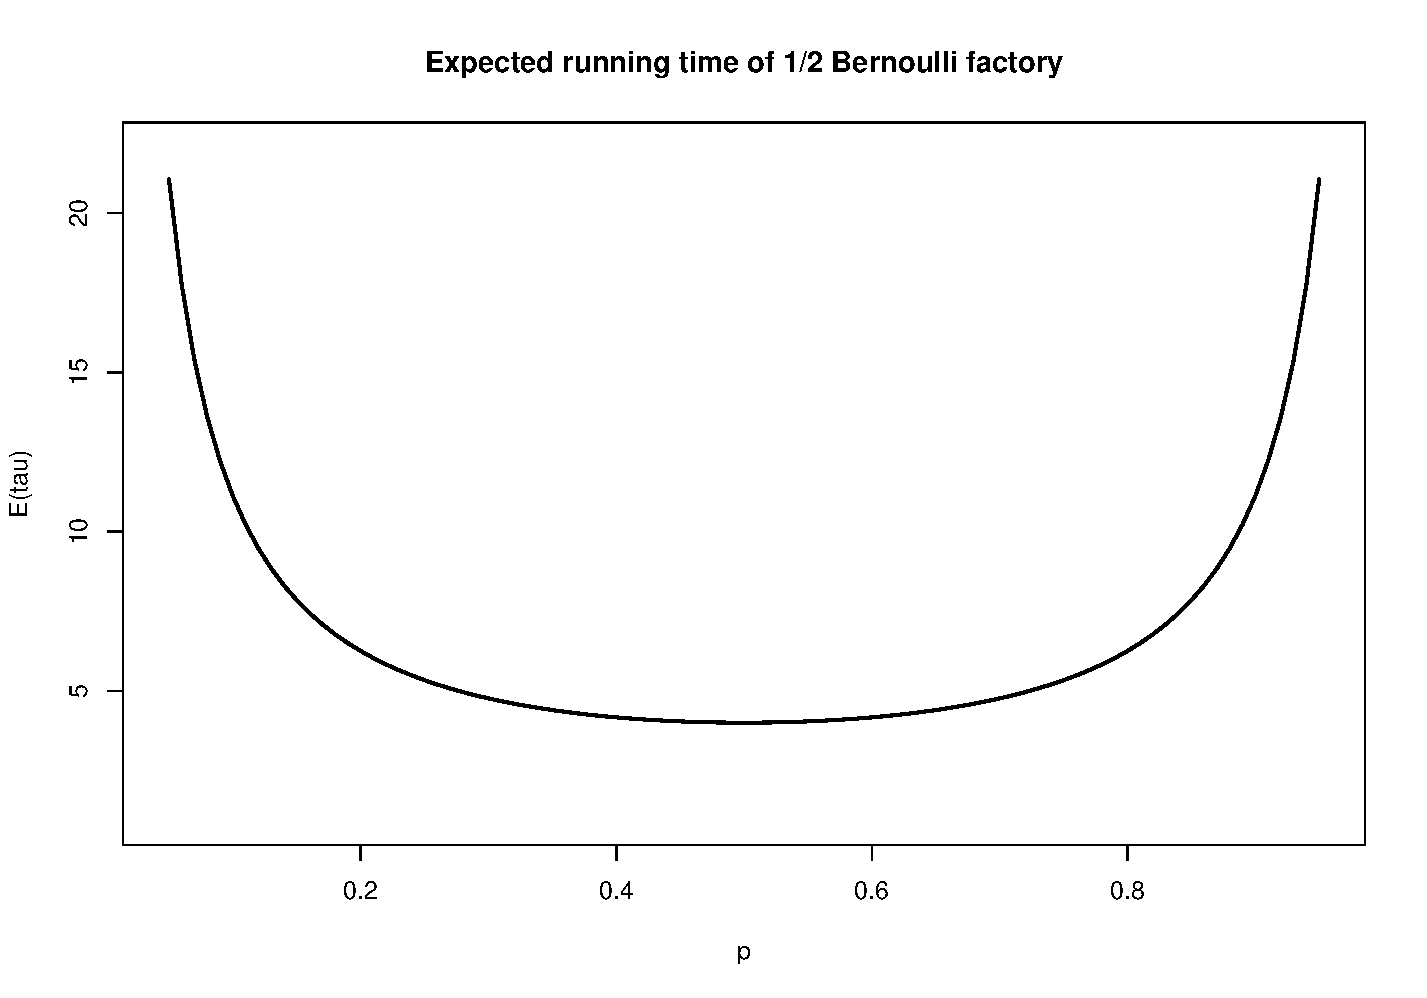
\includegraphics[width=0.8\textwidth]{vonneu_runtime.pdf}
\caption{Expected running time $\E(\tau)$ of von Neumann's Bernoulli factory for $f(p)\equiv 1/2$.  The expectation attains its minimum $\E(\tau)=4$ at $p=1/2$, and is moderate over a large range of $p$, but grows unboundedly as $p$ approaches 0 and 1.}
\label{fig:runtime_const2}
\end{figure}
\end{example}

The algorithm given in Example \ref{ex:const_half} can be extended to simulate other constant functions of the form $f(p)\equiv 1/k$ for $k\in \{2,3,\dots\}$. The generalised procedure is:
\begin{align*}
& \tau = \min\left\{ t \in \{k,2k,3k,\dots\} : \sum_{i=t-k+1}^t X_{i} = 1 \right\} \\
& \A(X_1,X_2,\dots) = X_\tau.
\end{align*}
However, the expected running time increases badly with $k$, even under certain early stopping strategies.

Of course, any constant $f(p)\equiv c$ is simulable by employing an auxiliary random variable $U\sim \Bern(c)$, but von Neumann's example shows that $c=1/2$ is also strongly simulable.
%N-P gives a procedure for any constant...
In fact, all constant functions are strongly simulable. The 1/2 procedure is a primitive for a Bernoulli factory for arbitrary constants $f(p)\equiv c\in[0,1]$, described in \citet[Proposition 13]{nacu2005}.

\begin{example}\label{ex:general_const}
$f(p)\equiv c\in[0,1]$ \\
We can write $c$ in its binary expansion
\begin{equation*}
c = \sum_{n=1}^\infty c_n 2^{-n}
\end{equation*}
where $c_n \in \{0,1\}$.
Using the procedure of Example \ref{ex:const_half} to generate (1/2)-coins, we toss (1/2)-coins until heads is observed. Call the number of (1/2)-coin tosses needed $M$. Finally we output $c_M$.
$M \sim \Geom(1/2)$, so the total probability of outputting heads is
\begin{equation*}
\PR(\text{heads}) = \sum_{n=1}^\infty \PR(\text{heads} \mid M=n) \PR(M=n) = \sum_{n=1}^\infty c_n \PR(M=n) = \sum_{n=1}^\infty c_n 2^{-n}
\end{equation*}
as desired.
The running time of this Bernoulli factory is $\tau \eqdist \Geom(1/2)\times 2 \times \Geom(2p(1-p))$, independent of $c$. So on average this procedure for a general constant takes twice as long as the procedure for 1/2.
\end{example}

Another important example is the case of $f(p)=p^2$, which is strongly simulable using exactly two queries, returning heads if and only if both inputs are heads. Example \ref{ex:bf_pk} presents a generalisation of this procedure.

\begin{example}\label{ex:bf_pk}
$f(p) = p^k, p\in[0,1], k\in\{1,2,\dots\}$.\\
This problem is solved easily by flipping the $p$-coin $k$ times and outputting heads if and only if all $k$ flips return heads. No auxiliary random variable is required.
\begin{align*}
& \tau = k \\
& \A(X_1,\dots,X_T) = \mathbb{I}\{X_1 =1, X_2=1 ,\dots,X_\tau=1\}
\end{align*}
It is clear that this procedure produces heads with probability $p^k$, since the flips are independent and each gives heads with probability $p$.

In this case the running time is deterministically equal to $k$. 
This can be decreased by an early stopping strategy, whereby we stop the process as soon as a tails input appears (in which case we know immediately that the output will be tails). In this case the running time is random, but still bounded above by $k$:
\begin{equation*}
\tau = k \wedge \min\{t \in \{1,2,\dots\}:X_t=0 \} \eqdist k \wedge \Geom(1-p).
\end{equation*}
Figure \ref{fig:p2_runtime} shows the expected running time of this procedure for a few values of $k$. We see that early stopping can significantly reduce the expected running time when $p$ is not close to 1, and that the gain in efficiency is greater for larger $k$. In the case $k=1$, where $f$ is the identity, the number of coin flips required is deterministically equal to 1, for any $p$.
\begin{figure}
\centering
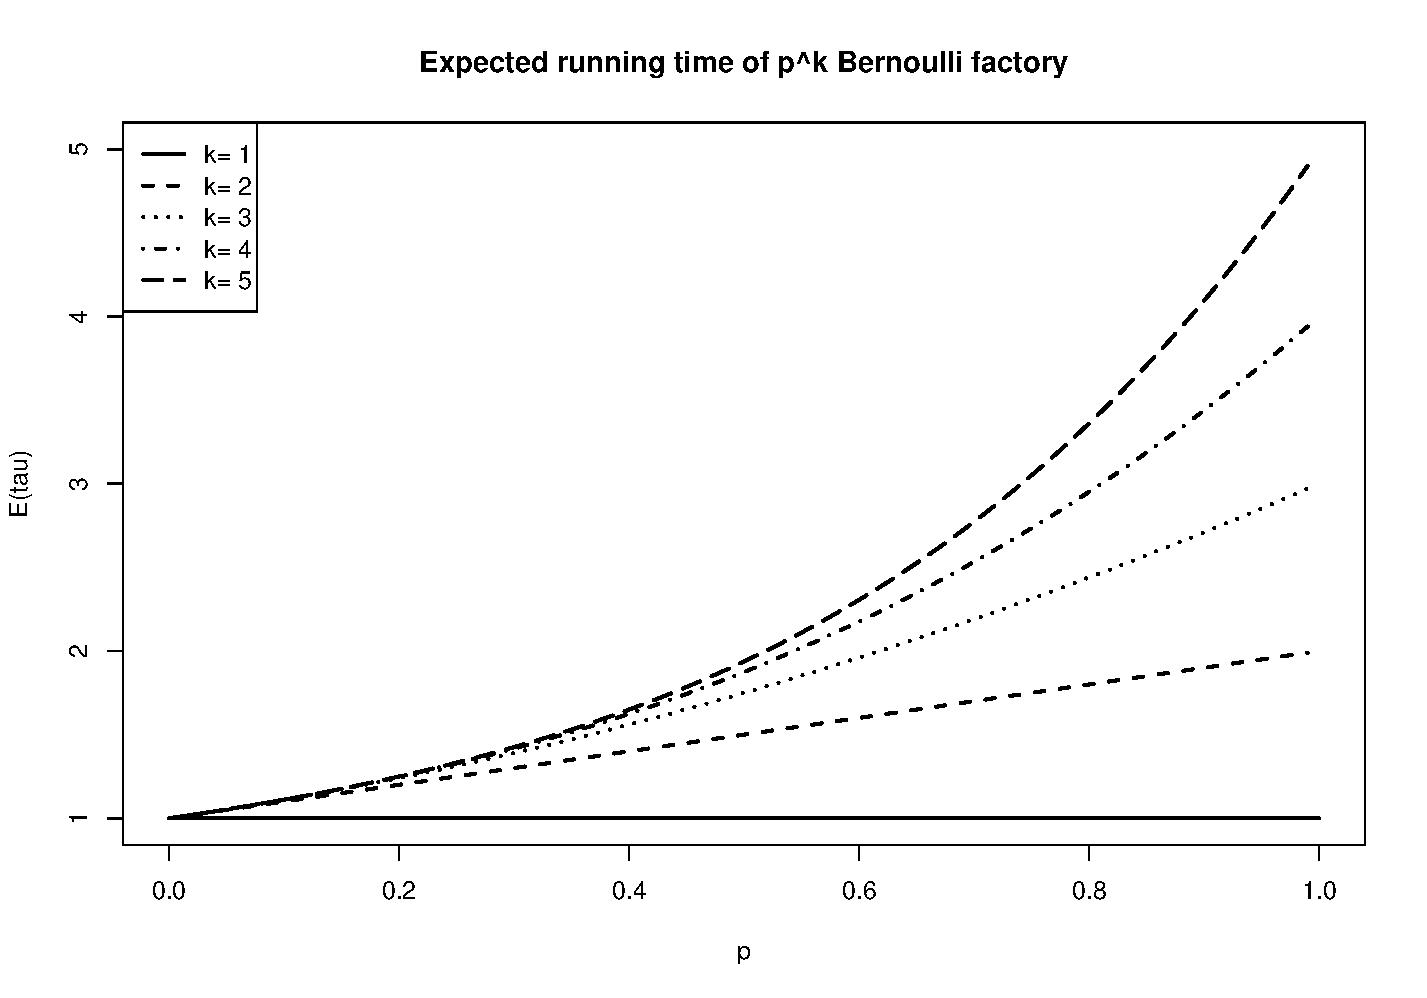
\includegraphics[width=0.8\textwidth]{pk_runtime.pdf}
\caption{Expected running time for the $f(p)=p^k$ Bernoulli factory with early stopping --- without early stopping, the running time is deterministically equal to $k$. The early stopping procedure significantly increases the efficiency, particularly when $p$ is small or $k$ is large. The minimum number of queries is one for all $k$ and $p$, and of course the $k=1$ (identity) Bernoulli factory requires exactly one query for any $p$.}\label{fig:p2_runtime}
\end{figure}
\end{example}

\begin{example}\label{ex:bf3}
$f(p) = 2p(1-p)$.\\
This is the probability of obtaining either 01 or 10 with two coin flips. Therefore the Bernoulli factory is simply:
\begin{align*}
& \tau = 2 \\
& \A(X_1,X_2) = \mathbb{I}\{(X_1,X_2) \in \{(0,1),(1,0)\} \}
\end{align*}
Of course, many other functions can be similarly obtained by varying the number of $p$-coin flips used and the set of inputs resulting in a heads output. One example, mentioned in \citet{patel2018}, is the function $f(p) = 3p(1-p)$. Noticing that $3p(1-p) = 3p^2(1-p) + 3p(1-p)^2$, this function is the probability of obtaining any outcome other than 000 or 111 with three coin flips.
\end{example}

Examples \ref{ex:const_half}--\ref{ex:bf3} cast some light on the sort of manipulations that are possible when constructing Bernoulli factories. Lemma \ref{thm:products_compositions} provides some general properties, all of which are trivial to prove.

\begin{lemma}\label{thm:products_compositions}
Suppose we have a Bernoulli factory $\A_f$ for the function $f:S_f\to[0,1]$ and a Bernoulli factory $\A_g$ for $g:S_g\to R_g\subseteq[0,1]$. Then
\begin{enumerate}[label=(\alph*)]
\item There exists a Bernoulli factory for $1-f: S_f \to [0,1]$, given by inverting the output of $\A_f$.
\item \label{thm:convex_combns} For any $\alpha \in [0,1]$ there exists a Bernoulli factory for $\alpha f + (1-\alpha) g$, given by first sampling from $\Bern(\alpha)$ and, depending on the outcome, using either $f$ or $g$.
\item \label{thm:compositions} If $R_g \subseteq S_f$, then there exists a Bernoulli factory for the composition $f\circ g: S_g \to [0,1]$, given by the composition $\A_f \circ \A_g$.
\item \label{thm:products} There exists a Bernoulli factory for the product $fg:S_f \cap S_g \to [0,1]$, given by $A_f \wedge A_g$.
\end{enumerate}
%In the case of \ref{thm:convex_combns}, \ref{thm:compositions} and \ref{thm:products} the overall running time is bounded if and only if the running time of both $A_f$ and $A_g$ is bounded.
\end{lemma}
Note that \ref{thm:convex_combns} is a special case of \ref{thm:compositions}.
Additionally, since there is a trivial Bernoulli factory for $f(p)\equiv 0$, \ref{thm:convex_combns} implies that $\alpha f$ is simulable for any $\alpha\in[0,1]$.
Many more properties, including consideration of their running times, are presented in \citet{nacu2005}.\\

It is not immediately obvious that not all functions are simulable. However, one counterexample is the following.
% f(p)=2p as canonical function = basis for constructing everything else [citation?]

\begin{example}\label{ex:2p}
$f(p) = 2p, p\in(0,1/2)$.\\
This function turns out not to be simulable, although the truncated function $f(p) = 2p \wedge (1-\varepsilon)$ --- or equivalently, restricting the domain to $p\in(0,(1 - \varepsilon)/2)$ --- is simulable for any $\varepsilon>0$. In this case the number of queries required is $O(\varepsilon ^{-1})$ \citep{huber2016}.

The problem with the unrestricted function is that $f(p)$ approaches 1 within $p\in(0,1)$, which violates one of the conditions given in the Keane-O'Brien theorem (Theorem \ref{thm:KOB}).
\begin{figure}
\centering
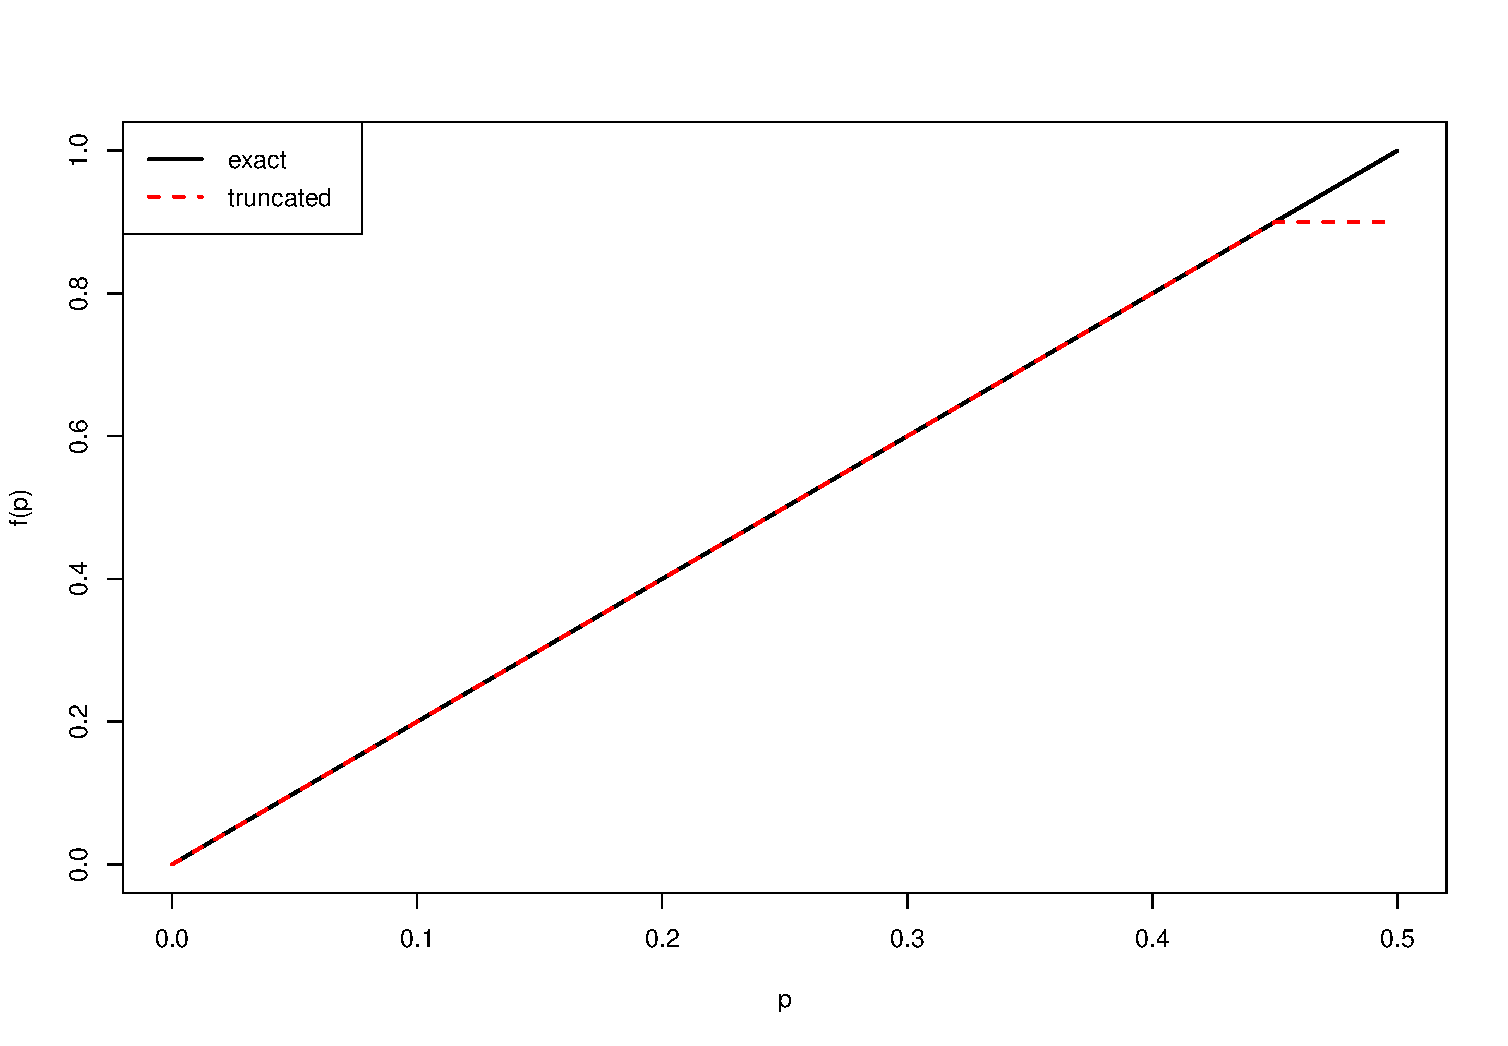
\includegraphics[width=0.8\textwidth]{2p_truncation.pdf}
\caption{The function $f(p)=2p$ (black) is not simulable; whereas the truncated function $f(p)=2p\wedge (1-\varepsilon)$ (red) is simulable for any $\varepsilon>0$, using $O(\varepsilon^{-1})$ queries.}
\label{fig:2p_truncation}
\end{figure}
\end{example}

\begin{lemma}\label{thm:no_2p_bf}
It is not possible to construct a Bernoulli factory for $f(p)=2p$ where $p\in(0,1/2)$.
\end{lemma}
The following proof is an intuitive one, adapted from \citet[Corollary 3.3]{latuszynski2011}.
The intuition behind the proof is that there is no sharp change between say a (1/4)-coin and a (1/2)-coin; but there is a qualitative difference between the resulting (1/2)-coin and 1-coin respectively. The latter is no longer random, but deterministically returns heads every time, regardless of the outcome on the (1/2)-coin that seeds it.
\begin{proof}
Let $\PR_{p}$ denote the probability measure conditioned on the input coin having probability $p$ of heads. We will compare the cases $p=1/4$ and $p=1/2 - \varepsilon$.
First, 
\begin{equation*}
\frac{1}{2} = \PR_{1/4} [\A(X_1,X_2,\dots)=0] = \lim_{t\to\infty} \PR_{1/4} [\A(X_1,\dots,X_T)=0, T<t]
\end{equation*}
Thus there exists a $t_0 \in \mathbb{N}$ such that 
\begin{equation*}
\PR_{1/4} [\A(X_1,\dots,X_T)=0, T\leq t_0] > \frac{1}{4}
\end{equation*}
%Now, fixing $\varepsilon>0$, consider the corresponding quantity $\PR_{1/2 - \varepsilon} [\A(X_1,\dots,X_T)=0, T\leq t_0]$; we have the following relation:
Bounding the maximum possible discrepancy between a sequence of $t_0$ flips from a $p$-coin and a (1/4)-coin, we have for any $p \in [1/4, 1/2)$:
\begin{equation*}
\PR_{p} [\A(X_1,\dots,X_T)=0, T\leq t_0] \geq \left(\frac{1}{2}\right)^{t_0} \PR_{1/4} [\A(X_1,\dots,X_T)=0, T\leq t_0] \geq \left(\frac{1}{2}\right)^{t_0+2}.
\end{equation*}
%%\texttt{Since, restricted to $T\leq t_0$, $\PR_p$ has the same support for any $p \in (0,1)$, we can consider the ratio of probabilities of any sequence in $\{0,1\}^{t_0}$. In particular, we consider 
%%\begin{equation*}
%%\inf_{p\in[1/4,1/2)}\, \inf_{A\subseteq\{0,1\}^{t_0}} \frac{\PR_{p}(A)}{\PR_{1/4}(A)}
%%\}end{equation*}
Now
\begin{equation*}
\PR_{1/2 - \varepsilon} [\text{output } 1] = 1-\PR_{1/2 - \varepsilon} [\A(X_1,X_2,\dots)=0]  \leq 1- \PR_{1/2 - \varepsilon} [\A(X_1,\dots,X_T)=0, T\leq t_0] \leq 1- \left(\frac{1}{2}\right)^{t_0+2}
\end{equation*}
Taking the limit as $\varepsilon\to 0$, the LHS is $f(1/2 - \varepsilon) = 1-2\varepsilon \rightarrow 1$, while the RHS is independent of $\varepsilon$ and remains strictly less than 1. This provides the contradiction, and hence such an algorithm $\A$ cannot exist.
\end{proof}
% not sure if this proof is complete and correct yet...

Lemma \ref{thm:no_2p_bf} is just a particular example of a general class of functions that cannot be simulated by a classical Bernoulli factory. The Keane-O'Brien theorem describes the exact class of classically simulable functions.
\begin{thm}[\citet{keane1994}]\label{thm:KOB}
A function $f:S\to[0,1]$ is simulable if and only if $f$ is continuous on $S$ and either
\begin{enumerate}[label=(\alph*)]
\item $f$ is constant on $S$, or
\item there exists $n\in\mathbb{N}$ such that $\min\{f(p),1-f(p)\} \geq \min\{p^n, (1-p)^n\}$ for all $p\in S$.
\end{enumerate}
\end{thm}

Roughly speaking, the second condition is ``$f(p)$ is polynomially bounded away from 0 and 1 inside its domain'' --- note that $f(p)$ is allowed to touch 0 and 1 at $p\in\{0,1\}$. A proof is given in \citet{keane1994}, but is not reproduced here. We now see that Lemma \ref{thm:no_2p_bf} follows as a corollary from the Keane-O'Brien theorem.
\begin{cor}
It is not possible to construct a Bernoulli factory for $f(p)=2p$ where $p\in(0,1/2)$.
\end{cor}
\begin{proof}
Firstly, $f$ is continuous on $S=(0,1/2)$, so the initial condition of Theorem \ref{thm:KOB} is satisfied.
Since $f$ is not constant, we require that there exists $n\in\mathbb{N}$ such that $\min\{f(p),1-f(p)\} \geq \min\{p^n, (1-p)^n\}$ for all $p\in S$.
Take $p=\frac{1}{2} - \varepsilon$; then $p\in S$ for all $\varepsilon>0$.
We calculate the relevant quantities and, since the inequality should hold for all $\varepsilon>0$,  we can take the limit $\varepsilon\to 0$:
\begin{align*}
&\min\{f(p),1-f(p)\} = 2\varepsilon \quad \overset{\varepsilon\to 0}{\longrightarrow}\quad 0 \\
&\min\{p^n, (1-p)^n\} = \left( \frac{1}{2} - \varepsilon \right)^n \quad \overset{\varepsilon\to 0}{\longrightarrow}\quad 2^{-n}.
\end{align*}
Since $2^{-n} >0$ for all $n\in\mathbb{N}$, we have that for all $n$ there exists $\varepsilon$ such that $\min\{f(p),1-f(p)\} < \min\{p^n, (1-p)^n\}$; therefore $f$ violates the second condition of Theorem \ref{thm:KOB}.
\end{proof}

\begin{thm}\label{thm:nacu_peres}
Let $f:S\to(0,1)$. 
There exists a Bernoulli factory for $f$ with $\tau$ satisfying the following properties, under the corresponding necessary conditions on $f$:
\begin{enumerate}[label=(\alph*)]
\item \label{thm:nplike_terminates_as} \textup{\citep{keane1994}} $\PR(\tau <\infty)=1$ only if $f$ is continuous on $S$.
\item \label{thm:np_finite_mean} \textup{\citep[Proposition 23]{nacu2005}} $\sup_{p\in S} \E(\tau) <\infty$, only if $f$ is Lipschitz over $S$. 
\item \label{thm:np_kth_moment} \textup{\citep[Proposition 22]{nacu2005}} $\E(\tau ^k)<\infty$ and $\lim_{n\to\infty} \E(\tau^k)\mathbb{I}\{\tau>t\} =0$ uniformly for all $p\in S$, only if $f$ is $k$ times continuously differentiable on $S$.
\item \label{thm:np_exponential_tails} \textup{\citep[Theorem 2]{nacu2005}} $\PR(\tau >t) \leq c\rho^t$, for some constants $c>0, \rho<1$ and for all $p\in S$, only if $f$ is real analytic on every open subset of $S$. %open/closed??? - different for each direction in N-P
\end{enumerate}
\end{thm}
%The conditions \ref{thm:np_exponential_tails} is referred to by \citet{nacu2005} as a ``fast'' simulation, but the term is used by someone else to mean something else...?
The four cases of Theorem \ref{thm:nacu_peres} are summarised in Table \ref{tab:theorems_summary}. Proofs are given in the original references but are not reproduced here.

\begin{table}
\centering
\begin{tabular}{l c l}
Property of $\tau$ & & Property of $f$ on $S$ \\
\hline
almost surely finite & $\Leftrightarrow$ & continuous \\
finite expectation & $\Leftarrow$ & Lipschitz \\
finite $k^{th}$ moment & $\Leftarrow$ & $k$ continuous derivatives \\
exponentially decaying tails & $\Leftrightarrow$ & real analytic
\end{tabular}
\caption{Summary of results from \citet{keane1994} and \citet{nacu2005} giving conditions on the function $f:S\to(0,1)$ for the existence of a Bernoulli factory with running time $\tau$ satisfying certain properties.}
\label{tab:theorems_summary}
\end{table}

\section{The quantum advantage}\label{sec:quantum_advantage}
It is known that for certain computational problems, quantum computers provide a theoretical advantage over classical computers. For instance, the Deutsch-Jozsa algorithm \citep{deutsch1992} is an example of a problem (if not a particularly practical one) which a quantum computer can solve in exponentially less time than the best possible classical algorithm.

It is widely believed (at least within the field) that quantum computing really is more powerful than its classical counterpart. Quantum computers are able to do anything that classical computers can, and quantum speed-ups have been proved for a handful of carefully constructed problems (see for another example Grover's algorithm for unstructured search \citep{grover1997}), so from a theoretical viewpoint there is no denying the so-called `quantum supremacy'.

There is, however, a lack of rigorous results for any computational problems with significant practical applications.
One such problem was apparently solved by \citet{kerenidis2016}, who came up with a quantum speed-up for the recommendation problem --- that is, how Amazon and Netflix estimate which products you will like given yours and other customers' ratings of all products. However, the authors were unable to prove that no comparably fast classical algorithm exists, and one has now been found \citep{tang2018}.

\subsection{Quantum Bernoulli factories}\label{sec:QBF}
The Bernoulli factory problem is an example of a practically applicable problem that is nevertheless simple to state and analyse. It was therefore a good candidate in the quest for a practical and provable quantum advantage, and indeed \citet{dale2015} prove this advantage. 

We will use the term \emph{quantum Bernoulli factory} to refer to an algorithm that takes (almost surely finitely many) $p$-quoins as inputs, and outputs a $\Bern(f(p))$ sample, where as usual $p\in S$ is unknown and $f:S\to [0,1]$ is known. A $p$-quoin is the quantum analogue of a classical $p$-coin, given by the quantum state
\begin{equation*}
\ket{p} = \sqrt{1-p}\, \ket{0} + \sqrt{p}\, \ket{1}.
\end{equation*}
This is a sensible definition since measuring $\ket{p}$ in the computational basis gives output 0 with probability $1-p$ or 1 with probability $p$, like a classical $p$-coin.
Note that the quantum Bernoulli factory has a quantum input (quoins) and a classical output (measurement outcome).
We will call a function \emph{quantum simulable} if there exists a quantum Bernoulli factory to simulate it.

\citet{dale2015} prove that quantum computation allows a strictly larger class of functions to be simulated than in the classical setting, taking as an example the notorious $f(p)=2p$. While this function is not simulable classically, the authors show that it is quantum simulable, and provide an explicit algorithm using two entangled qubits.
They also determine necessary and sufficient conditions (Theorem \ref{thm:qbf_simulable}) for a function to be quantum simulable, which are weaker than those in the Keane-O'Brien theorem (Theorem \ref{thm:KOB}).

% CBFs subset of QBFs (Dale eqn 1)

\begin{thm}[{\citet[Theorem 1]{dale2015}}]\label{thm:qbf_simulable}
A function $f:[0,1]\to[0,1]$ % can say S\to[0,1] as above ??
is quantum simulable (using only operations on single qubits) if and only if:
\begin{enumerate}[label=(\alph*)]
\item $f$ is continuous on S
\item $Z:=\{z:f(z)=0\}$ and $W:=\{w:f(w)=1\}$ are both finite sets
\item\label{thm:qbf_cond_zeroes} $\forall z\in Z$ there exist constants $c\in\mathbb{R}$, $\delta>0$, integer $k<\infty$ such that $c(p-z)^{2k} \leq f(p)$ for all $p \in [z-\delta, z+\delta]$
\item\label{thm:qbf_cond_ones} $\forall w\in W$ there exist constants $c\in\mathbb{R}$, $\delta>0$, integer $k<\infty$ such that $1 - c(p-w)^{2k} \leq f(p)$ for all $p \in [w-\delta, w+\delta]$.
\end{enumerate}
\end{thm}
In the quantum case, the function $f$ is allowed to touch 0 and 1 at finitely many points in its domain, as opposed to the classical case where $f(p)$ may only take the values 0 and 1 at $p\in\{0,1\}$ or in the cases of the constant functions $f\equiv 0$ and $f\equiv 1$.
The conditions \ref{thm:qbf_cond_zeroes} and \ref{thm:qbf_cond_ones} ensure that $f$ goes to 0 or 1 only polynomially quickly at these points.

\citet{dale2015} also claim that the same necessary and sufficient conditions apply even when operations on more than one qubit are allowed. That is, taking advantage of quantum entanglement (as in Section \ref{sec:qbf_2p}) does not expand the set of simulable functions. It can, however, substantially reduce the consumption of $p$-quoins, as demonstrated in \citet{patel2018}.


\subsection{A quantum Bernoulli factory for 2p}\label{sec:qbf_2p}
This section describes the quantum algorithm of \citet{dale2015} for the function $f_\wedge(p) := 2\min\{p, 1-p\}$, $p\in[0,1]$. This function (Figure \ref{fig:wedge_fn}) coincides with that of Example \ref{ex:2p} when the domain is restricted to $p\in(0,1/2)$, so it is sufficient to find a Bernoulli factory for $f_\wedge$.

Although \citet{dale2015} also construct a quantum algorithm using only measurements on single qubits (and both algorithms are implemented by \citet{patel2018}), we will focus on the two-qubit algorithm which is simpler to describe and gives the best performance.

First note that 
\begin{equation}\label{eq:2p_seriesexp}
f_\wedge(p) = 2\min\{p, 1-p\} = 1-\sqrt{1-4p(1-p)} = \sum_{k=1}^{\infty} \binom{2k}{k} \frac{1}{(2k-1)2^{2k}} (4p(1-p))^k =: \sum_{k=1}^{\infty} q_k (4p(1-p))^k
\end{equation} % check that taylor expansion /!\
where $q_k$ are constants not depending on $p$, and are therefore simulable. Due to property \ref{thm:convex_combns} of Lemma \ref{thm:products_compositions}, $f_\wedge$ is then simulable if there exists a Bernoulli factory for $(4p(1-p))^k$. Since this is a case of Example \ref{ex:bf_pk}, we need only construct a Bernoulli factory for $4p(1-p)$. This function is not classically simulable since it still touches 1 at $p=0.5$ (Figure \ref{fig:wedge_qbf_fn}).

% add flow diagram or pseudocode for the full algorithm

However, \citet{dale2015} describe the following quantum Bernoulli factory for the function $4p(1-p)$.
We first prepare two $p$-quoins; that is, we have two qubits jointly in the product state $\ket{p}\ket{p}$. We then measure the joint state in the (entangled) Bell basis, say with the operator
\begin{equation*}
0\cdot\ket{\phi^+}\bra{\phi^+} + 1\cdot\ket{\phi^-}\bra{\phi^-} + 2\cdot\ket{\psi^+}\bra{\psi^+} + 3\cdot\ket{\psi^-}\bra{\psi^-}.
\end{equation*} 
The possible measurement outcomes are:
\begin{align*}
&\PR(\text{observe }0) = \braket{v|\phi^+}\braket{\phi^+|v} = 1/2 \\
&\PR(\text{observe }1) = \braket{v|\phi^-}\braket{\phi^-|v} = \frac{(1-2p)^2}{2} \\
&\PR(\text{observe }2) = \braket{v|\psi^+}\braket{\psi^+|v} = 2p(1-p) \\
&\PR(\text{observe }3) = \braket{v|\psi^-}\braket{\psi^-|v} = 0
\end{align*}
This means that $\PR(\text{observe }1 \text{ or } 2) = 1/2$, and $\PR(\text{observe } 2 \mid \text{observe }1 \text{ or } 2) = 4p(1-p)$, which is the required function.
Thus our Bernoulli factory for $4p(1-p)$ is as follows: measure $\ket{p}\ket{p}$ in the Bell basis until the observed outcome is either 1 or 2, then return heads if the outcome is 2, or tails if the outcome is 1. 
This procedure has running time $\tau \eqdist \Geom(1/2)$, which has exponentially decaying tails.

Let us now consider the full procedure for $f_\wedge$.
We first choose a $k$ according to the probability distribution $\{q_k\}$ (Figure \ref{fig:qbf_qk}).
We then repeat the the $4p(1-p)$ Bernoulli factory $k$ times to determine the output. The full procedure therefore has running time 
\begin{equation*}
\tau \eqdist \Geom(1/2) \sum_{k=1}^\infty k \cdot q_k
\end{equation*}
which is almost surely finite as required. But since $k\cdot q_k$ is not summable, the \emph{expected} running time is $\E(\tau)=+\infty$ for all $p$.

However, we can improve the running time by using early stopping as in Example \ref{ex:bf_pk}, so that we output tails as soon as any of the $4p(1-p)$ procedures outputs tails. In this case the running time becomes 
\begin{equation*}
\tau \eqdist \Geom(1/2) \sum_{k=1}^\infty [\Geom(1-4p(1-p)) \wedge k] \cdot q_k.
\end{equation*} 
Conditioned on the choice of $k$, the expectation is
\begin{equation*}
\E(\tau \mid k) = 2\cdot \frac{1-(4p(1-p))^k}{1-4p(1-p)}.
\end{equation*}
The unconditional expectation is not available analytically, but an approximation is shown in Figure \ref{fig:qbf_wedge_runtime}.
The Geometric early stopping time moderates the overall running time sufficiently that it has finite expectation whenever $p\neq 1/2$, but $\E(\tau) \to +\infty$ as $p\to 1/2$. That is, the algorithm behaves badly around the `difficult' point $p=1/2$.

\begin{figure} % combine these onto one plot?
\centering
\begin{subfigure}{0.45\linewidth}
\centering
\includegraphics[width=\textwidth]{wedge_function.pdf}
\caption{The function $f_\wedge(p)$}
\label{fig:wedge_fn}
\end{subfigure}%
\hfill
\begin{subfigure}{0.45\linewidth}
\centering
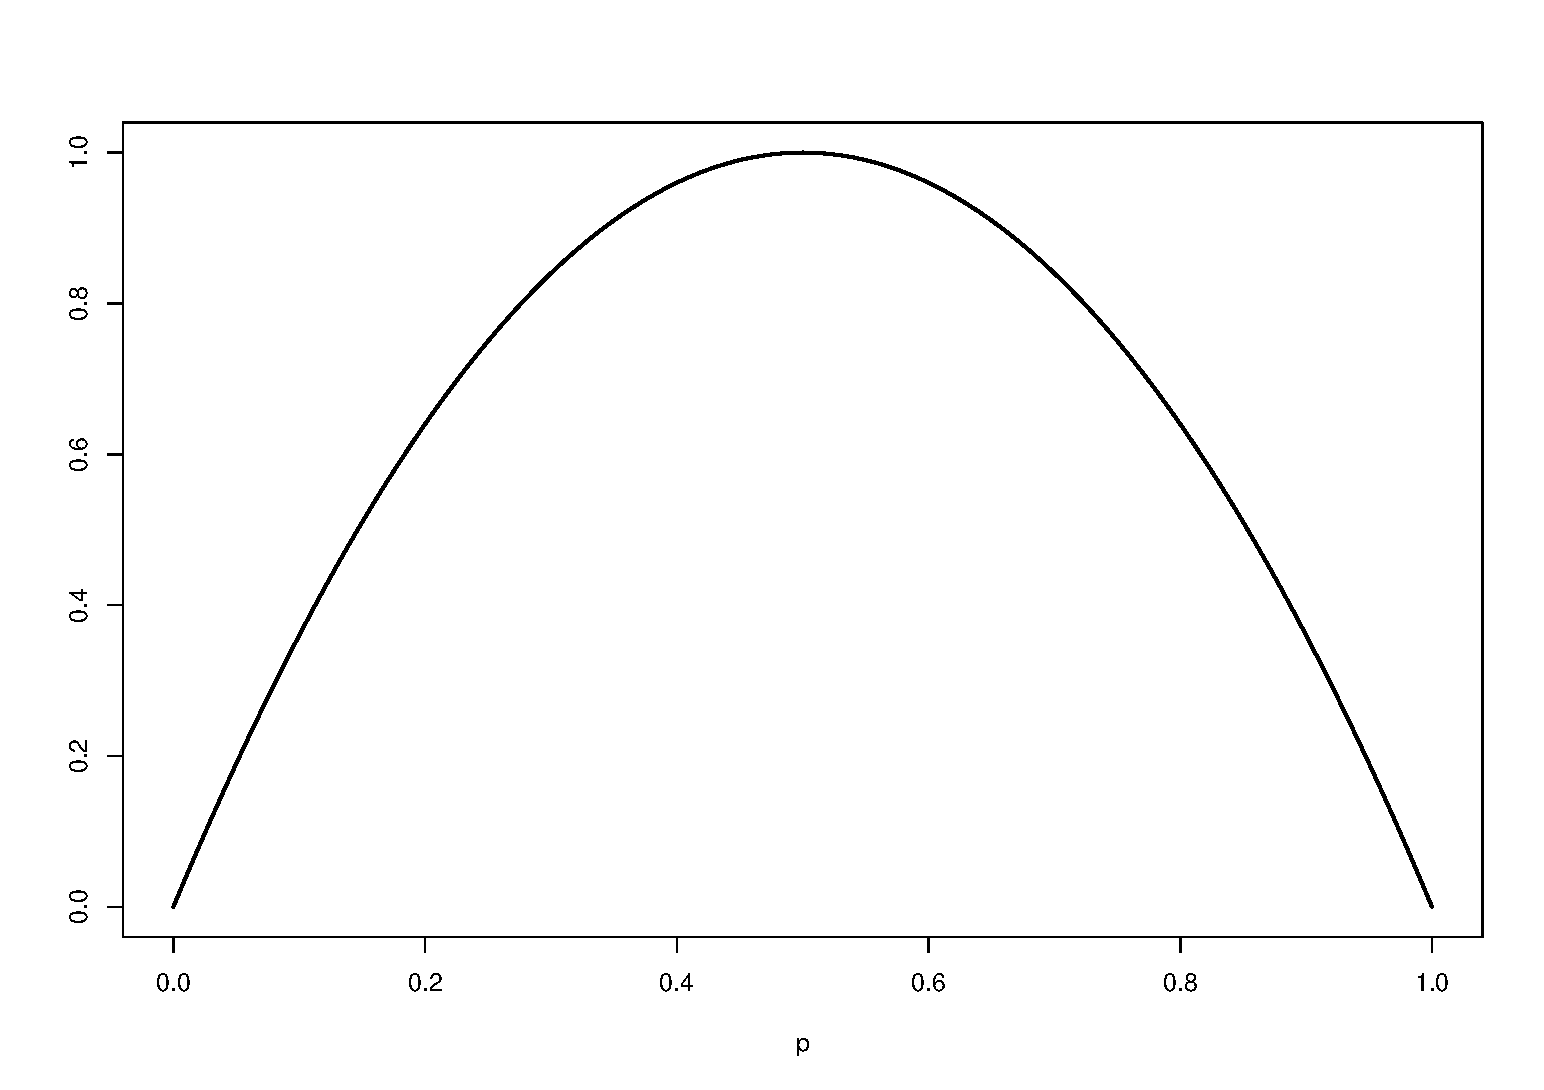
\includegraphics[width=\textwidth]{wedge_qbf_fn.pdf}
\caption{The function $4p(1-p)$}
\label{fig:wedge_qbf_fn}
\end{subfigure}
\caption{The function $f\wedge(p)=2\min\{p, 1-p\}$ cannot be simulated classically since it touches 1 within its domain. Simulation of $f_\wedge(p)$ reduces to simulation of $4p(1-p)$, which is also classically unobtainable, but is quantum simulable.}
\end{figure}

\begin{figure}
\centering
\begin{subfigure}{0.45\linewidth}
\centering
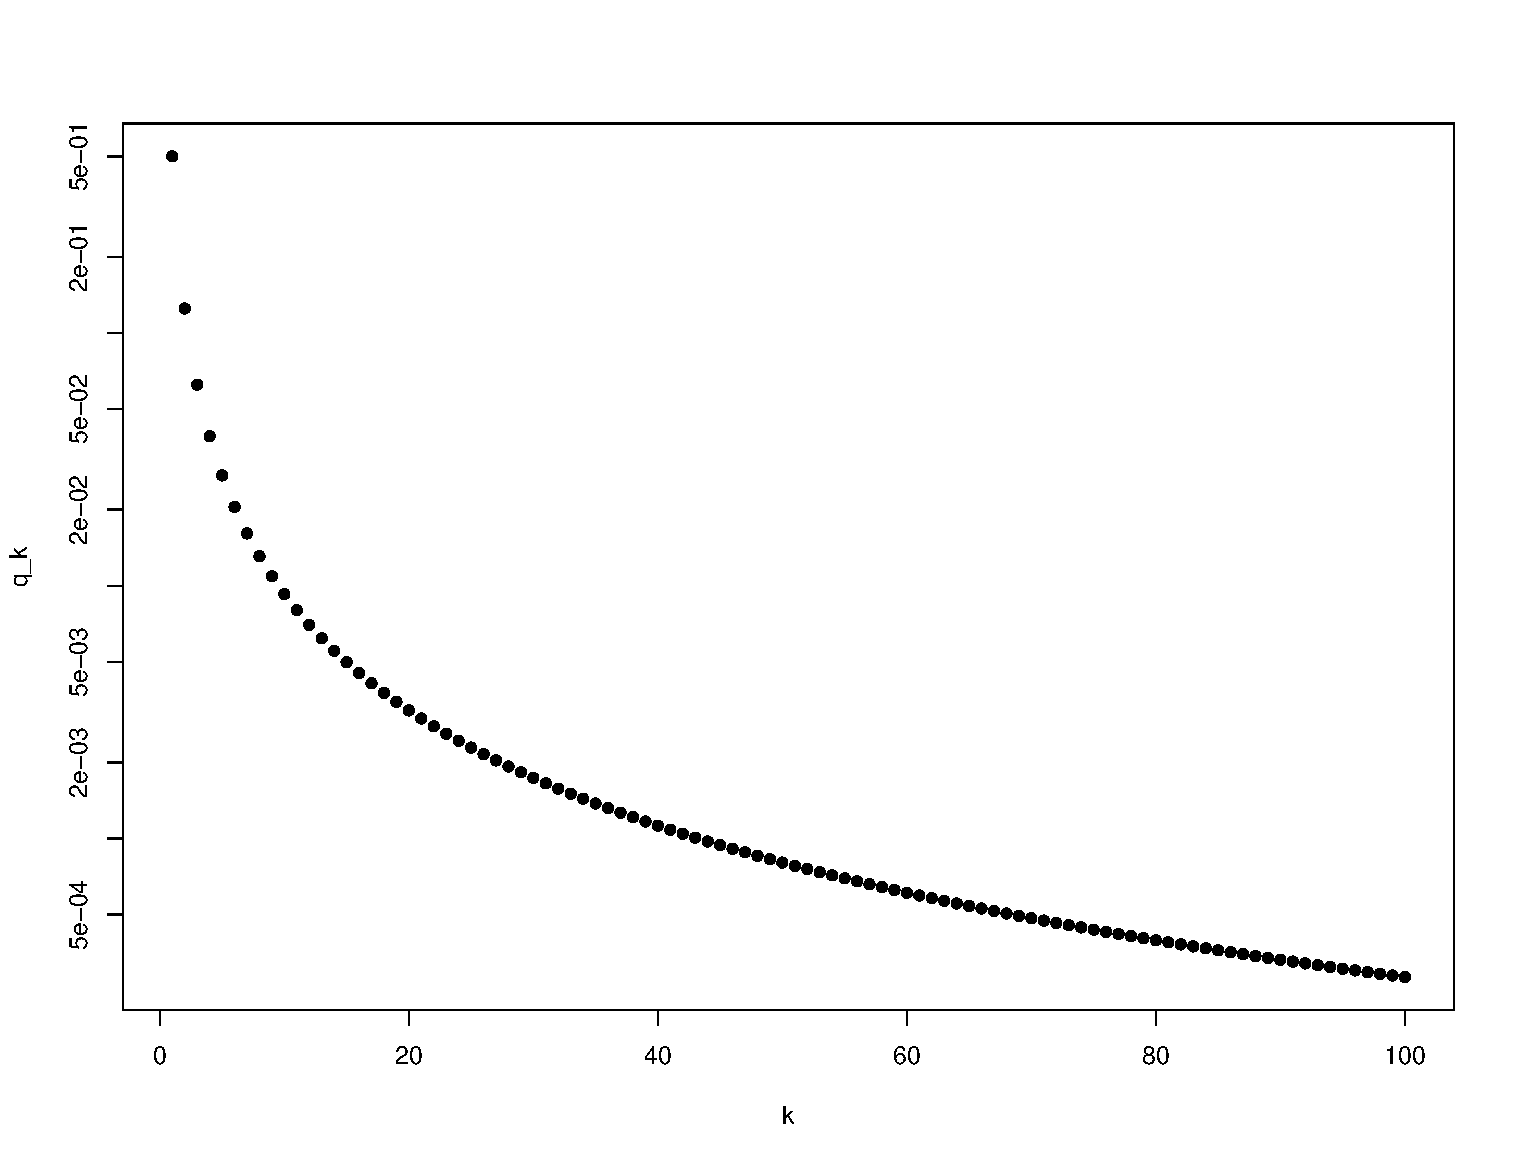
\includegraphics[width=\textwidth]{qk_values.pdf}
\caption{Value of $q_k$ (on a logarithmic scale) for various $k$. The probabilities decay quickly, so it is unlikely to choose a large value of $k$ which would make the quantum Bernoulli factory slow.}
\label{fig:qbf_qk}
\end{subfigure}%
\hfill
\begin{subfigure}{0.45\linewidth}
\centering
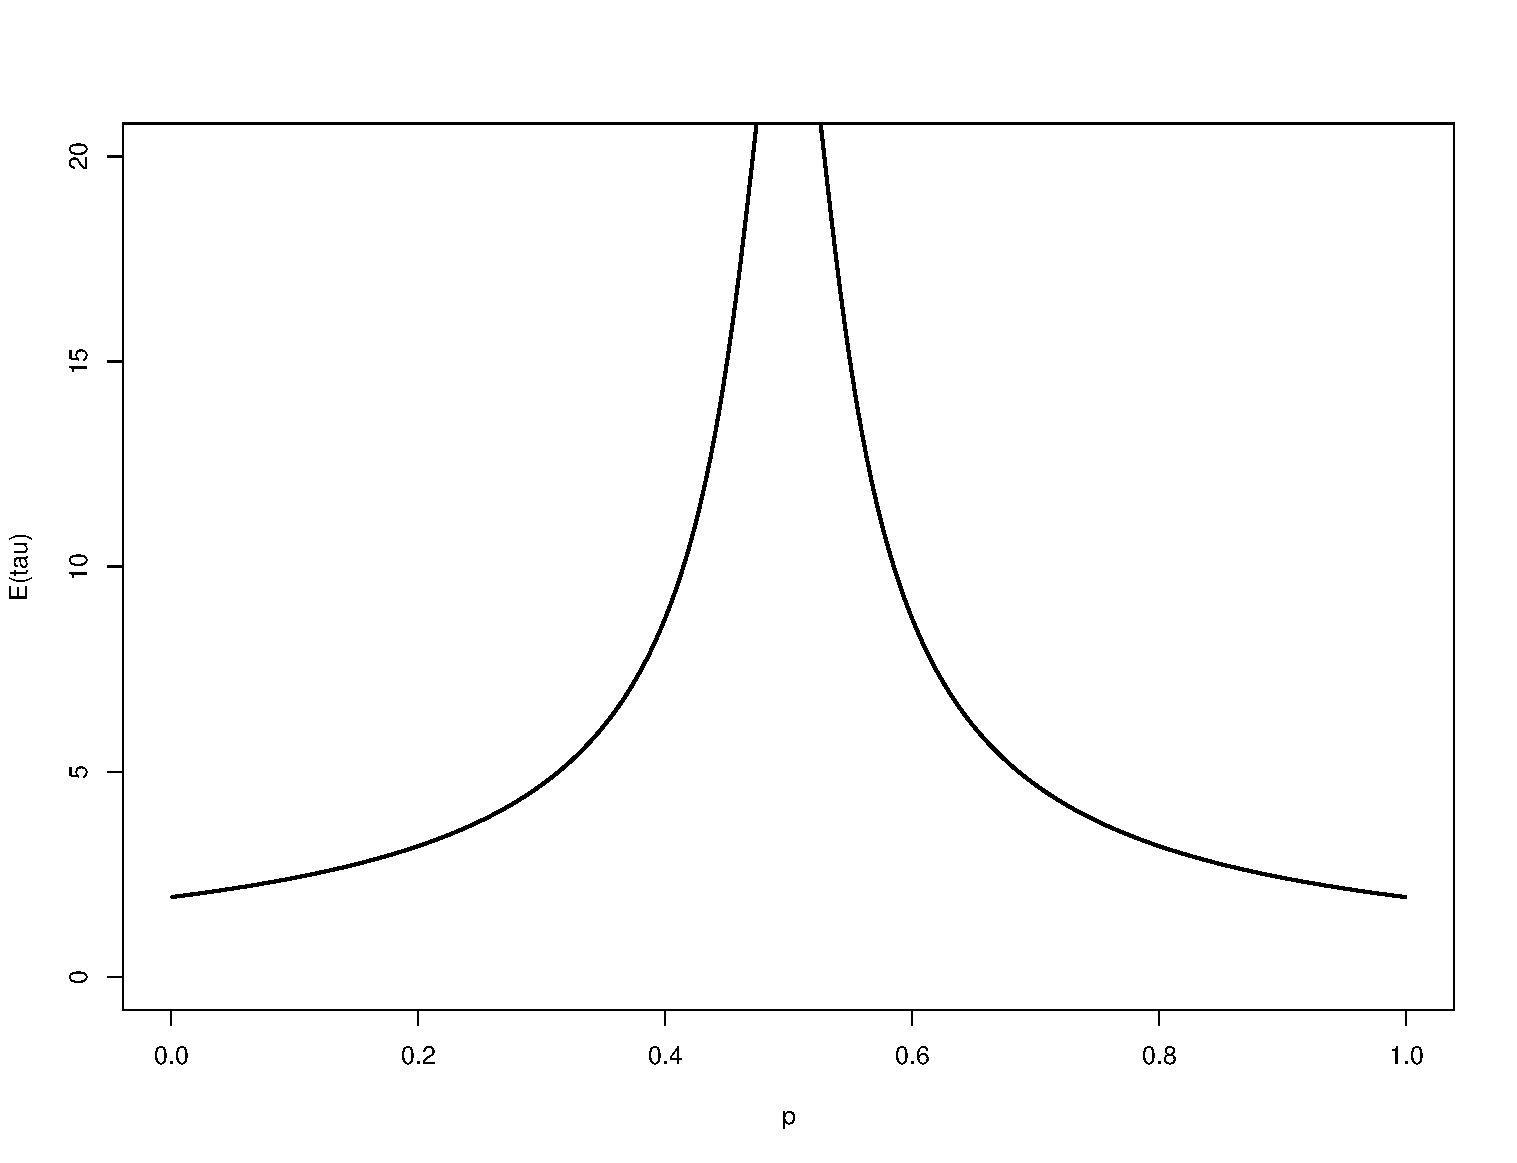
\includegraphics[width=\textwidth]{2p_qbf_runtime.pdf}
\caption{Expected running time for the $f_\wedge(p)$ quantum Bernoulli factory. The running time is almost surely finite for all $p$, but its expectation goes to infinity when $p$ is close to 1/2.}
\label{fig:qbf_wedge_runtime}
\end{subfigure}
\caption{(a) Value of $q_k$ for $k=1,\dots, 100$. (b) Expected running time of the QBF for $f_\wedge(p)$.}
\end{figure}

\begin{figure}
\centering
\includegraphics[width=0.8\textwidth]{approxtarget_1520100500.pdf}
\caption{Approximations to $f_\wedge(p)$ when the series expansion \eqref{eq:2p_seriesexp} is truncated at $k_{max} = 1,5,20,100,500$. Each subsequent approximation is closer to the target function, but none attains the ideal $f(1/2)=1$.}
\label{fig:qbf_target_approximations}
\end{figure}

\subsubsection{Experimental considerations}
\citet{patel2018} describe a physical implementation of this quantum Bernoulli factory. 
Since in a physical system infinite quoin consumption cannot be allowed, the authors approximate the infinite series \eqref{eq:2p_seriesexp} by truncating it after $k_{max}$ terms. The resulting target functions are only approximations of $f_\wedge$, which are rounded at the top and therefore do not touch 1 at $p=1/2$ (Figure \ref{fig:qbf_target_approximations}). %\citep[Figures 3a--d]{patel2018}.

In fact, the authors admit that with the experimental equipment currently available, it is not possible to achieve a better approximation than that given by $k_{max} \simeq 2000$; for higher-order approximations, the experimental errors become overwhelming. This means that there is a bound on the maximum experimental precision of the quantum algorithm, no matter how many quoins we are allowed to use --- a shortcoming not suffered by the classical algorithm. Of course, improvements in equipment will allow higher precision, but it is reasonable to suppose that it will always be bounded at some level.

Also, the authors do not run their experiment at the input value $p=1/2$, presumably since the coin consumption there would ideally have infinite mean and so the experiment would be time-consuming, with many runs using the maximum $k_{max}$ quoins.
\citet[Figure 3e]{patel2018} shows a realisation of the quoin consumption, similar to Figure \ref{fig:qbf_wedge_runtime}, except that in practice the quoin consumption cannot approach infinity, and tops out at a mean of 60 in their experiment, when $p$ is close to 1/2.

This raises a question as to whether the quantum Bernoulli factory for $f_\wedge$ is really an improvement on the classical truncated one, since experimental constraints effectively amount to something like an $\varepsilon$-truncation of the function even in the quantum case (Figure \ref{fig:qbf_target_approximations}).
However, \citet{patel2018} claim that the quantum algorithm given a fixed number of input quoins achieves a much better approximation than the best classical algorithm using the equivalent number of input coins. This is investigated further in Section \ref{sec:scaling}.

\subsubsection{Scaling limits}\label{sec:scaling}
\citet{huber2016} shows that the best classical Bernoulli factory for $f(p)=2p\wedge 1-\varepsilon$ has running time that scales like $1/\varepsilon$, where $\varepsilon$ is the error at $p=1/2$ between the ideal function $f(p)=2p$ and the approximate (truncated) function.
In the quantum case we can similarly define $\varepsilon$ as the error at $p=1/2$ between $f_\wedge$ and the approximation using $k_{max}$ terms in the series expansion \eqref{eq:2p_seriesexp}.

Figure \ref{fig:eps_scaling} shows the theoretical relationship between expected quoin consumption (running time) and approximation error $\varepsilon$, for $p$ close to 1/2 (recall that at $p=1/2$ the running time has infinite expectation).
The approximation error is given by
\begin{equation*}
\varepsilon = 1 - \sum_{k=1}^{k_{max}} q_k
\end{equation*}
and the expected quoin consumption is
\begin{equation*}
\frac{2}{1-4p(1-p)} \sum_{k=1}^\infty q_k [1-(4p(1-p))^k].
\end{equation*}
Each black point represents a different value of $k_{max}$, from 1 (bottom right) to 500 (top left). The value of $p$ used is 0.499; bringing $p$ any closer to 0.5 makes no perceptible difference. The red line shows the fitted $\E(\tau) \propto 1/\varepsilon$ relationship, which appears to fit the data very well.

\citet{patel2018} claim that the quoin consumption scales like $\varepsilon^{-1/2}$, but their result is obtained by averaging over all values of $p$. This seems an unfair comparison, since the scaling is worst close to $p=1/2$. Indeed if the equivalent Figure \ref{fig:eps_scaling} is produced for different values of $p$ we see much better scaling when $p$ is not close to 1/2, so averaging over $p$ favourably biases the results.
The classical scaling result of \citet[Theorem 1]{huber2016} considers the `worst-case' of the running time, taking the supremum over $p$, which is what we have tried to emulate here.

It seems therefore that both the classical and quantum Bernoulli factories for $2p$ have running time that scales with $1/\varepsilon$ when $p$ is close to 1/2. This suggests that the huge experimental difference in resource usage observed by \citet{patel2018} must be due only to better constants in the quantum case.

\begin{figure}
\centering
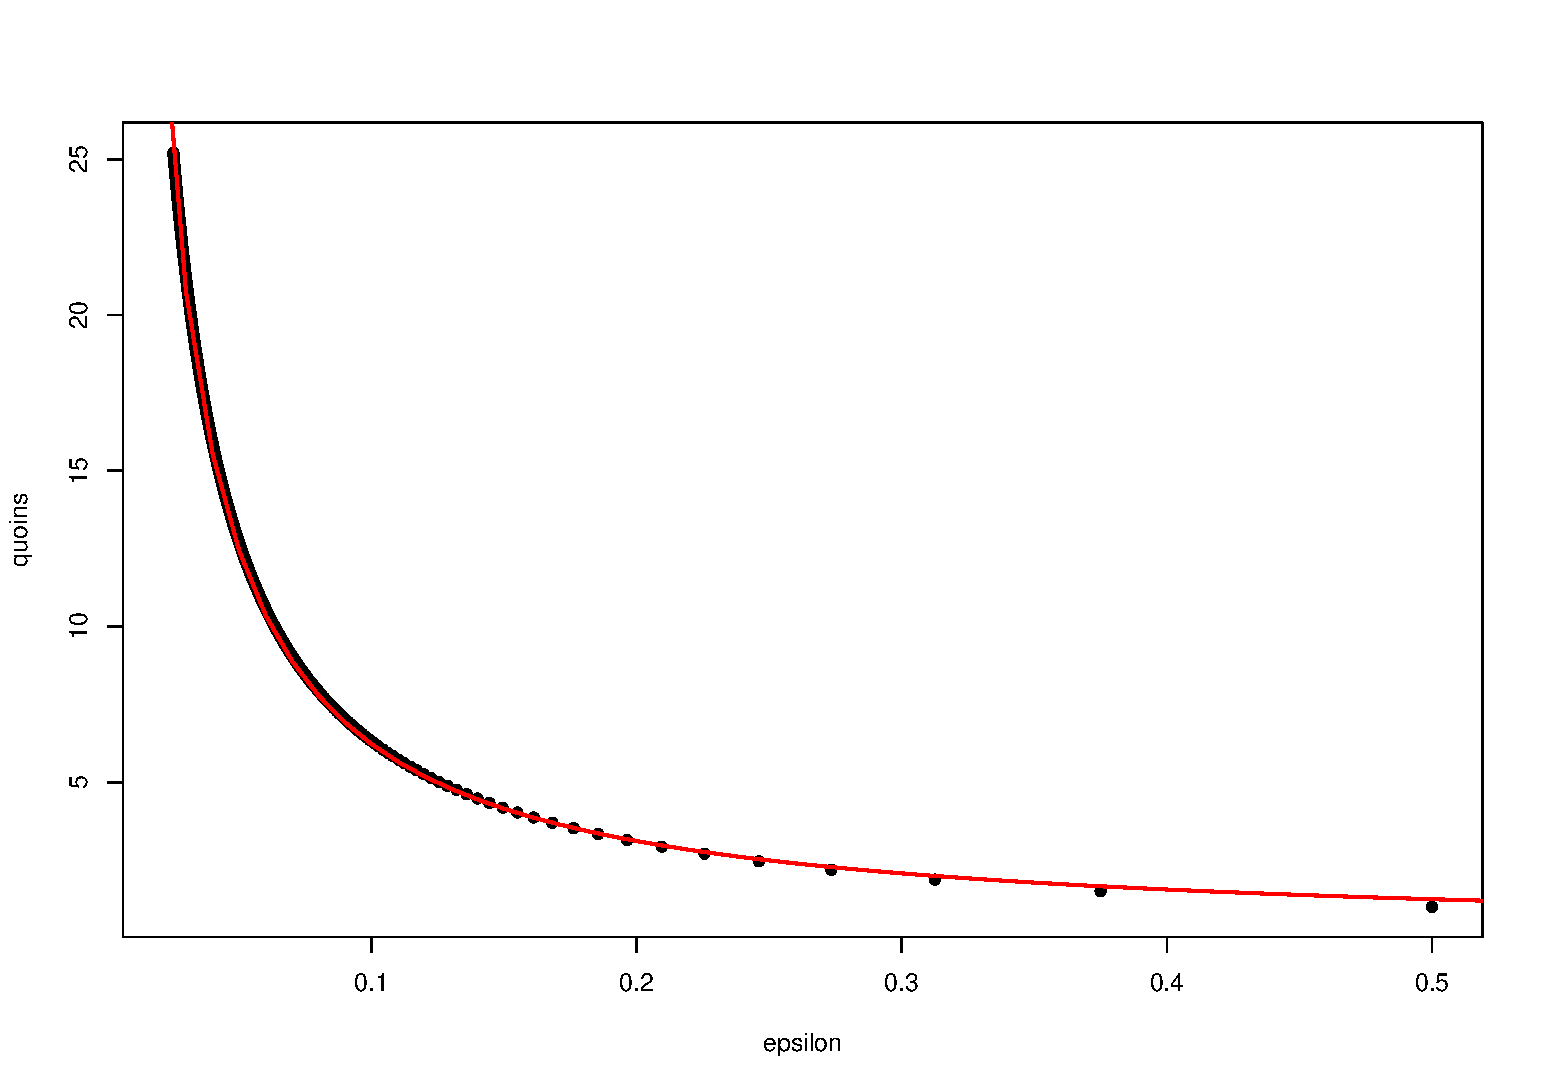
\includegraphics[width=0.8\textwidth]{eps_scaling.pdf}
\caption{Expected running time (quoin consumption) at $p=0.499$ of the quantum Bernoulli factory for $f_\wedge$, for various values of $k_{max}$ from 1 (bottom right) to 500 (top left), against the amount of error $\varepsilon$ incurred by truncating at $k_{max}$ terms. A $1/\varepsilon$ relationship (red line) seems to fit very well.}
\label{fig:eps_scaling}
\end{figure}


\subsection{Another quantum Bernoulli factory}
A more impressive, if less fundamentally important, example is obtained by considering the function
\begin{equation*}
h_a(p) := \left( \sqrt{p(1-a)} - \sqrt{a(1-p)} \right)^2
\end{equation*}
which is plotted for various values of $a$ in Figure \ref{fig:function_ha}.
This function is not classically simulable except when $a\in\{0,1\}$, since it takes the value 0 when $p=a$. (Note that for $a\in\{0,1\}$ we simply recover the functions $p$ and $1-p$ respectively, which are trivially simulable using one coin.)
On the other hand, $h_a(p)$ is quantum simulable for all $a\in[0,1]$. Moreover, it can be simulated by a quantum Bernoulli factory using just one quoin.
The quantum procedure involves applying the unitary operator
\begin{equation*}
\begin{pmatrix}
\sqrt{1-a} & \sqrt{a} \\
-\sqrt{a} & \sqrt{1-a}
\end{pmatrix}
\end{equation*}
to a $p$-quoin $\ket{p} := \sqrt{1-p}\,\ket{0} + \sqrt{p}\,\ket{1}$, producing the state
\begin{equation*}
\left( \sqrt{(1-a)(1-p)} + \sqrt{ap} \right) \ket{0}
+ \left( \sqrt{p(1-a)} - \sqrt{a(1-p)}\right) \ket{1}.
\end{equation*}
Measurement in the computational basis then outputs 1 with the desired probability $h_a(p)$.

This is an example of how the quantum ability to manipulate quoins prior to measurement yields flexibility that is not available through classical processing.
The function $h_a(p)$ is used in \citet{dale2015} to produce upper and lower bounding functions for $f(p)$, which are required to construct generic quantum Bernoulli factories and prove Theorem \ref{thm:qbf_simulable}.

\begin{figure}
\centering
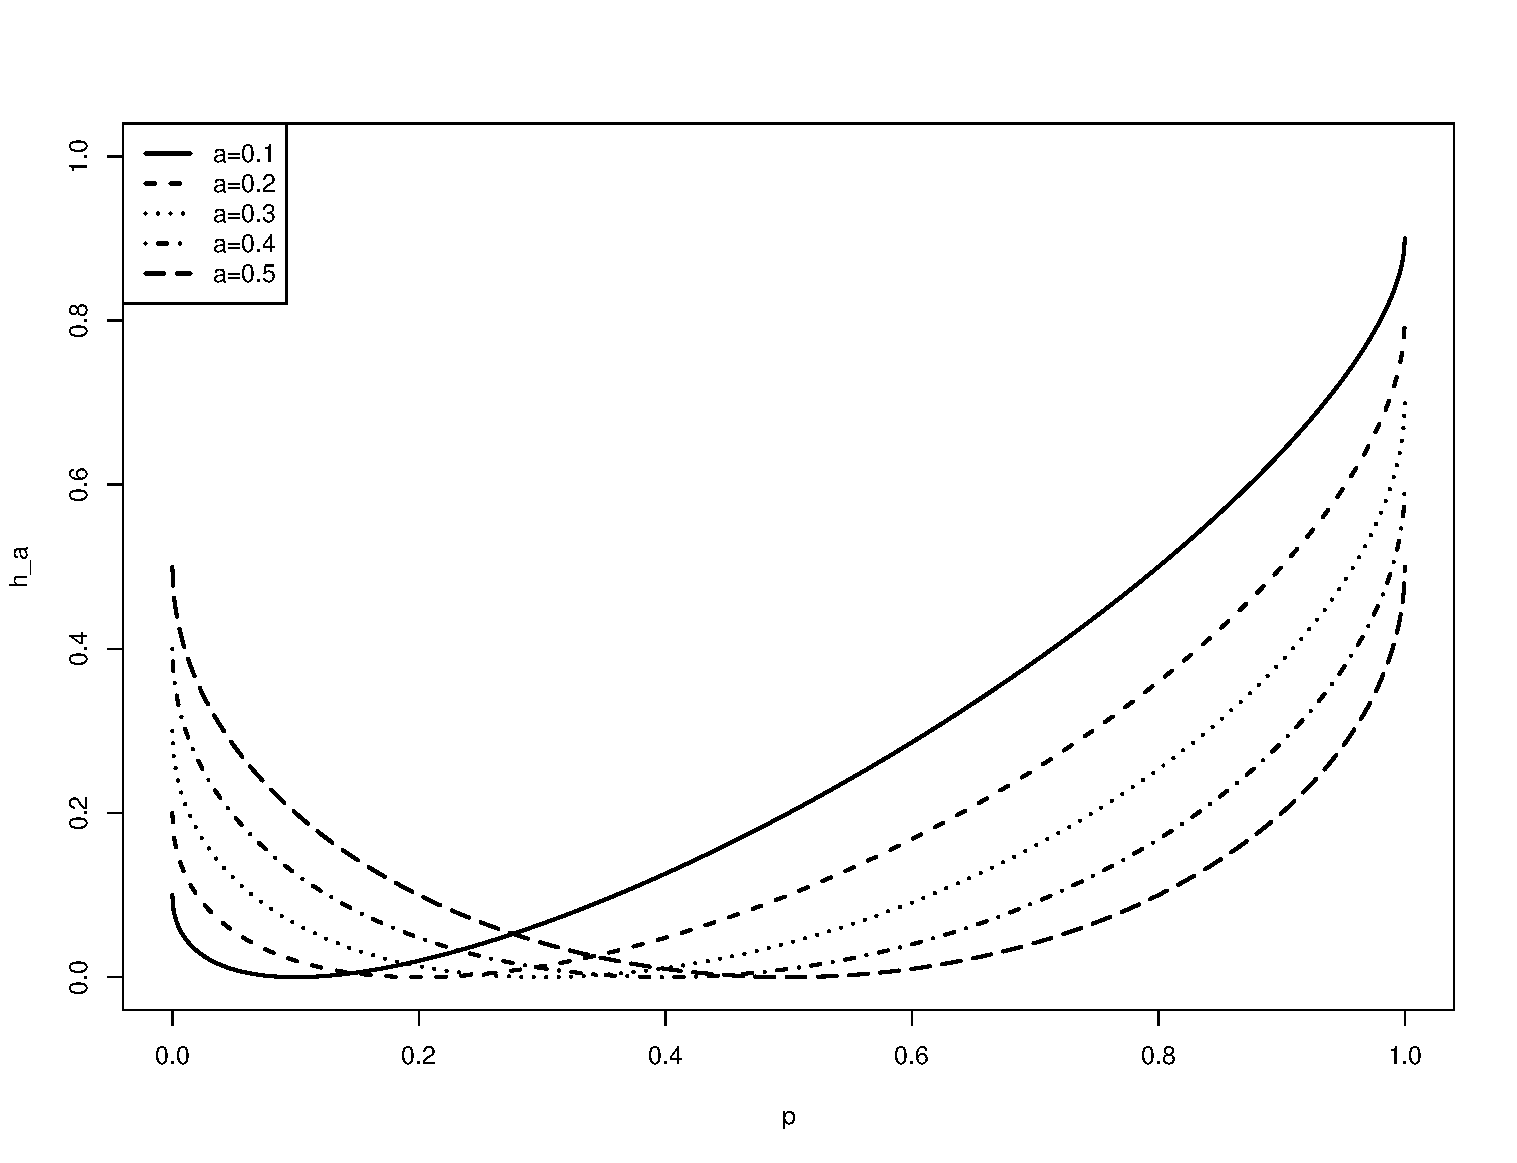
\includegraphics[width=0.8\textwidth]{function_ha.pdf}
\caption{The function $h_a(p)$ for various values of $a$ (taking $a>0.5$ produces the reflection in $p=0.5$ of $h_{1-a}$). These functions are not classically simulable except for $a\in\{0,1\}$ because they touch 0 at $p=a$. But they can be simulated by a quantum Bernoulli factory using just one $p$-quoin.}
\label{fig:function_ha}
\end{figure}


\section{Discussion}\label{sec:discussion}
We have seen necessary and sufficient conditions describing the exact class of functions that are simulable by classical and quantum Bernoulli  factories respectively.
The class of classically simulable functions is a strict subset of the class of quantum simulable functions, proving the superiority of quantum computing in this application.

For the purposes of comparison we took a $p$-quoin, as the quantum analogue of a $p$-coin, to be equal in value to a classical $p$-coin flip.
However this comparison does not seem particularly fair. 
Firstly, the running time of the quantum Bernoulli factory is measured as the number of $p$-quoins consumed, whereas the running time of the classical Bernoulli factory is the number of flips of a $p$-coin used. In a sense, the classical Bernoulli factory only requires a single coin which can be flipped many times, while in the quantum Bernoulli factory a quoin is produced and destroyed at every step.
But this is still not quite the right way to look at it, since the classical coin is an abstraction and does not really exist; there are only Bernoulli samples which, like the quoins, are `used up' at each step.

The second and more serious issue is that constructing a $p$-quoin requires the value of $p$ to be available (though not necessarily known to the experimenters). That is, producing the quantum state $\ket{p}$ requires a quantum computer to take the value of $p$ as an input \citep{hebdige2018} --- but the fundamental point of a Bernoulli factory is that $p$ is unknown.

On a philosophical level, we can abstract the problem and imagine that in both the classical and quantum cases $p$ is unknown to the experimenters but known to some third party. That third party is then responsible in the classical case for feeding the value of $p$ into a Bernoulli sample generator, or in the quantum case for feeding $p$ into a $p$-quoin generator. In this framework, $p$ plays the same role for both factories. This framework also addresses the first problem, because we can then equate classical coins with `dephased' quoins, which are exactly like quoins except that they lack the ability for quantum coherence and entanglement.

However, this sort of abstraction neglects the original purpose of our Bernoulli factory. Returning to the Monte Carlo setting, we want to use a Bernoulli factory to decide whether to accept or reject a proposal during a particular step of a Metropolis-Hastings algorithm. The objective is to accept with probability exactly equal to $\alpha$, where $\alpha$ is a function of $p$. 
The value of $p$ itself is not available analytically, nor can it be estimated efficiently. We are only able to draw samples from $\Bern(p)$, and it may be computationally expensive to do so.

Such samples are precisely the inputs required by a classical Bernoulli factory, so in the case of classically simulable functions they are sufficient to produce an exact sample from $\Bern(\alpha)$. On the other hand, the quantum Bernoulli factory requires the value of $p$ as an input, which is a much stronger requirement. The only possibility is to use many $\Bern(p)$ samples to produce an estimate of $p$ from which to construct quoins, in which case the Bernoulli factory would only be approximate.

In light of these caveats, it seems that the quantum Bernoulli factory is not after all the coveted applicable example of quantum supremacy, but just another toy problem with no important application. The ``provable quantum advantage'' appears only when the classical coins are taken to be `dephased' quoins, in which case the algortihms are no longer applicable to Monte Carlo simulation.

\bibliography{qbf.bib}
\end{document}